\documentclass[a4paper,12pt,headsepline]{scrartcl}

%\part{title}
\usepackage[utf8]{inputenc}
\usepackage{graphicx}
\usepackage{caption,subcaption}
\usepackage[main=english, ngerman]{babel}
\usepackage[T1]{fontenc}
\usepackage{geometry}
\usepackage{proof}
\geometry{left=3.5cm, right=3.5cm, top=2.5cm, bottom=2cm}
\usepackage{hyperref}
%\usepackage[hyphens,obeyspaces,spaces]{url}
\usepackage{fancybox}
\usepackage{amssymb,amsmath,amsthm}
\usepackage{gensymb}
\usepackage[linesnumbered,ruled,vlined,norelsize]{algorithm2e}
%\usepackage[bookmarksnumbered,pdftitle={\titleDocument},hyperfootnotes=false]{hyperref} 
\usepackage{color}
\usepackage{float}

\usepackage{datetime}

\newdateformat{myformat}{\THEDAY{. }\monthname[\THEMONTH], \THEYEAR}

%test
\usepackage[backend=biber]{biblatex}
% \usepackage{filecontents}

\addbibresource{ref.bib}

\restylefloat{figure}

% Makros
\newenvironment{sketch}{\begin{proof}[Proof (Sketch)]}{\end{proof}}
\newtheorem{theorem}{Theorem}
\newtheorem{assumption}{Assumption}
\newtheorem{lemma}{Lemma}
\newtheorem{remark}{Remark}
\newtheorem{definition}{Definition}
\newtheorem{observation}{Observation}
\newtheorem{corollary}{Corollary}
\newcommand{\comment}[1]
{
  \begin{quotation}
    \textcolor{blue}{\underline{Edit:} #1}
  \end{quotation}
}
\newcommand{\TODO}[1]
{
  \begin{quotation}
    \textcolor{red}{\underline{TODO:} #1}
  \end{quotation}
}
\newcommand{\mygraphics}[3][2]{
\begin{figure}[h]
	\centering
	\includegraphics[page=#1]{#2}
	\caption{#3}
\end{figure}
}

% Zeichen 
\newcommand{\Rho}{\ensuremath{\mathcal{O}}}
\newcommand{\ec}{\texttt{ec}}
\newcommand{\NP}{\call{NP}}
\newcommand{\call}[1]{\ensuremath{\mathcal{#1}}}
\newcommand{\UL}{\texttt{UL}~}

% neue Kopfzeilen mit fancypaket
\usepackage{fancyhdr} %Paket laden
\pagestyle{fancy} %eigener Seitenstil
\fancyhf{} %alle Kopf- und Fußzeilenfelder bereinigen
\fancyhead[L]{\nouppercase{\leftmark}} %Kopfzeile links
\fancyhead[C]{} %zentrierte Kopfzeile
\fancyhead[R]{\thepage} %Kopfzeile rechts
\renewcommand{\headrulewidth}{0.4pt} %obere Trennlinie
%\fancyfoot[C]{\thepage} %Seitennummer
%\renewcommand{\footrulewidth}{0.4pt} %untere Trennlinie

\frenchspacing
\makeindex

% Pseudocode für Java
\usepackage{listings}
\lstset{numbers=left, numberstyle=\tiny, numbersep=5pt, keywordstyle=\color{black}\bfseries, stringstyle=\ttfamily,showstringspaces=false,basicstyle=\footnotesize,captionpos=b}
\lstset{language=python}

% Disable single lines at the start of a paragraph (Schusterjungen)
\clubpenalty = 10000
% Disable single lines at the end of a paragraph (Hurenkinder)
\widowpenalty = 10000
\displaywidowpenalty = 10000

\begin{document}
\newpage
\thispagestyle{empty} % erzeugt Seite ohne Kopf- / Fusszeile
\section*{ }
%Seitennummerierung römisch
\pagenumbering{roman} 
% das Papierformat zuerst
%\documentclass[a4paper, 11pt]{article}

% deutsche Silbentrennung
%\usepackage[ngerman]{babel}

% wegen deutschen Umlauten
%\usepackage[ansinew]{inputenc}

% hier beginnt das Dokument
%\begin{document}


\thispagestyle{empty}

%\begin{figure}[t]
% \centering
% \includegraphics[width=0.6\textwidth]{abb/logo1}
%~~~~~~~~~~
% \includegraphics[width=0.3\textwidth]{abb/logo2}
%\end{figure}


\begin{verbatim}


\end{verbatim}

\begin{center}
\Large{Eberhard Karls Universität Tübingen}\\
\small Wilhelm Schickard Institut Tübingen\\
\end{center}


\begin{center}
\Large{Fachbereich Informatik}
\end{center}
\begin{verbatim}




\end{verbatim}
\begin{center}
%\doublespacing
\textbf{\LARGE{On euclidian distances in drawings of certain graph classes (Working Title)}}\\
%\singlespacing
\begin{verbatim}

\end{verbatim}
\textbf{{Arbeitsbereich Algorithmik}}
\end{center}
\begin{verbatim}

\end{verbatim}
\begin{center}

\end{center}
\begin{verbatim}

\end{verbatim}
\begin{center}
\textbf{zur Erlangung des akademischen Grades \\ Master of Science}
\end{center}
\begin{verbatim}






\end{verbatim}
\begin{flushleft}
\begin{tabular}{llll}
\textbf{Autor:} & & Benjamin \c Coban & \\
& & MatNr. 3526251 & \\
& & \\
\textbf{Version vom:} & & \foreignlanguage{ngerman}{\myformat\today} &\\
& & \\
\textbf{ErstprüferIn:} & & Prof. Dr. Michael Kaufmann &\\
\textbf{ZweitprüferIn:} & & Prof. Dr. Ulrike von Luxburg &\\
\end{tabular}
\end{flushleft}
\section*{Zusammenfassung}
%Firstly, we show that every Kandinsky drawing of arbitrary degree can be postprocessed to a smooth orthogonal drawing and planarity is preserved. As a base for postprocessing a Kandinsky drawing, we use the \textit{Fixed Shape Model}, which preserves the orientation of the vertices. The area bounds of SMOGs are $\Rho(n^2)\times\Rho(n)$ in the worst case. The complexity of a polyedge \textit{does not increase} if and only if the polyedge is \textit{purely uniform} and rise to $\left\lfloor\frac{3}{2}k\right\rfloor$ if and only the the polyedge is \textit{purely alternating}. In practice, it is possible that a polyedge contains several uniform and alternating parts. The \textit{fragmentation} of a polyedge delivers a mathematical description in order to examine all kinds of situations. With help of the optimal fragmentation, we can guarantee that a rather \textit{high complexity} of a polyedge in the original Kandinsky drawing \textit{only increases to} $k+2$.
Graphenzeichnungen sind vielfältig in ihrer Anwendung - im Bezug auf VLSI Design oder Metroliniennetz sind \textit{orthogonale} Zeichnungen besonders relevant. Dies bedeutet, dass jede Kante als Abfolge von horizontalen und vertikalen Liniensegmenten, welche rechtwinklig an sogenannten \textit{Knicken} aneinander knüpfen, dargestellt wird. Ein weitverbreitetes Modell ist das sogenannte \textit{Kandinsky Modell}. Die \textit{Glättung} solcher Zeichnungen arbeitet zusätzlich mit Viertelkreissegmenten, sodass die Ecken abgerundet werden. Dabei ist das Verhalten der sogenannten \textit{Komplexität} der Kanten - aus wievielen Segmenten solch eine Kante in der geglätteten Zeichnung nun besteht - zu untersuchen.
\\\\
Im ersten Abschnitt der Ausarbeitung werden wir zeigen, dass die Glättung einer Kandinsky Zeichnung möglich ist. Ist die Eingangszeichnung kreuzungsfrei, so bleibt diese Eigenschaft erhalten. Die Ausrichtung der Knoten wird dabei nicht grundlegend verändert. Allerdings wird dabei die geglättete Zeichnung größer - der horizontale Platzverbrauch kann sich im schlimmsten Fall quadrieren. Die Komplexität der Kanten bleibt bei ausgehenden Kandinsky Zeichnungen überschaubar. Besteht eine Kante aus mehr als vier Segmenten, erhöht sich deren Komplexität um zwei. 
\\\\
Im nächsten Abschnitt beschäftigen wir uns mit verschiedenen Ansätzen, um an Platzverbrauch und Kantensegmenten der resultierenden Zeichung zu sparen. Wir zeigen einen Ansatz, um den horizontalen Platzverbrauch $b$ im besten Fall auf $\sqrt{b}$ zu schrumpfen. Weiter wird eine Kombination aus Kreis- und Liniensegmenten vorgeschlagen, sodass der horizontale Platzverbrauch sich nur um den Wurzelwert $\sqrt{b}$ vervielfacht.
\\\\
In weiterführender Arbeit wird schließlich durch eine Gadgetkonstruktion gezeigt, dass es \textit{\NP-hart }ist zu entscheiden, ob ein Graph mit einer geglätteten Zeichnung ohne Knicke illustriert werden kann. \textit{Achtelkreissegmente} werden auf ihre Eigenschaften untersucht, da sie relevant für weiterführende Projekte sein können.
%In the next section we figure out several approaches in order to \textit{decrease} the complexity of edges and the area bounds of the smooth orthogonal drawings. A \textit{modified plane sweep} can save up to $\Rho(n)$ area and is able to save some horizontal segments. This plane sweep suits as a handy approach to optimize given SMOG drawings. Further we show an alternative to circular arcs - a \textit{combination} of a quarter arc and a vertical segment increases the complexity, but only needs $\sqrt{r}$ width relative to the original quarter arc.

%Finally, we show a \textit{gadget construction} as a \textit{reduction} from the \NP-hard \textit{SAT problem} to a bendless SMOG with arbitrary degree. \textit{Octi arcs} may be relevant for further work - e.g. illustration of graphs with at most one crossing per edge - and are examined for its properties.
\section*{Abstract}
%Graphenzeichnungen sind vielfältig in ihrer Anwendung - im Bezug auf VLSI Design oder Bahnliniennetz sind \textit{orthogonale} Zeichnungen besonders relevant. Dies bedeutet, dass jede Kante als Abfolge von Liniensegmenten, welche rechtwinklig an sogenannten \textit{Knicken} aneinander knüpfen, dargestellt wird. Ein weitverbreitetes Modell ist das sogenannte \textit{Kandinsky Modell}. Die \textit{Glättung} solcher Zeichnungen arbeitet zusätzlich mit Viertelkreissegmenten, sodass die Ecken abgerundet werden. Dabei ist das Verhalten der sogenannten \textit{Komplexität} der Kanten - aus wievielen Segmenten solch eine Kante in der geglätteten Zeichnung nun besteht - zu untersuchen.
Graph drawings are diverse in their applications - considering VLSI or metro map design, \textit{orthogonal} drawings are of interest. In an orthogonal drawing, every edge is illustrated as a sequence of axis-aligned line segments which intersect in a point, so-called \textit{bends}. This thesis will examine one of the most common models of orthogonal drawings - the \textit{Kandinsky model}. The \textit{smoothening} of such Kandinsky drawings introduces circular quarter arc segments for smoothening the 90\degree~angles. The behaviour of the \textit{complexity} of such an edge - the amount of segments illustrating a smoothened edge relative to the orthogonal case - is to examine. 
\\\\
First, we will show the possibility of smoothening Kandinsky drawings. Several properties of the drawings are preserved. If the input drawing is crossing-free, the smoothened drawing will also be crossing-free and the orientation of the vertices is not mainly altered. However, the smoothened drawing may increase in size - the horizontal area consumption may be squared in the worst case. The complexity of input Kandinsky drawings may not significantly rise. If the input edge consists of at least four segments, then the complexity of the smoothened edge increases by two.
%Im ersten Abschnitt der Ausarbeitung werden wir zeigen, dass die Glättung einer Kandinsky Zeichnung möglich ist. Ist die Eingangszeichnung kreuzungsfrei, so bleibt diese Eigenschaft erhalten. Die Ausrichtung der Knoten wird dabei nicht grundlegend verändert. Allerdings wird dabei die geglättete Zeichnung größer - der horizontale Platzverbrauch kann sich im schlimmsten Fall quadrieren. Die Komplexität der Kanten bleibt bei ausgehenden Kandinsky Zeichnungen überschaubar. Besteht eine Kante aus mehr als vier Segmenten, erhöht sich dessen Komplexität um zwei. 
\\\\
Next, several approaches in order to save segments and area consumption are established. A method is shown, how to shrink the horizontal area consumption by its square root in the best case. A combination of circular arc and line segments is introduced to reduce the area expansion in the smoothened drawing.
%Im nächsten Abschnitt beschäftigen wir uns mit verschiedenen Ansätzen, um an Platzverbrauch und Kantensegmenten der resultierenden Zeichung zu sparen. Wir zeigen einen Ansatz, um den horizontalen Platzverbrauch $b$ im besten Fall um $\sqrt{b}$ zu schrumpfen. Weiter wird eine Kombination aus Kreis- und Liniensegmenten vorgeschlagen, sodass der horizontale Platzverbrauch sich nur um den Wurzelwert $\sqrt{b}$ vervielfacht.
\\\\
In the extensional work, a gadget construction is introduced to prove the \textit{\NP-hardness} whether a given graph admits a \textit{bendless} smoothened drawing. \textit{Eighth circular arc segments} - or \textit{octi arcs} - are examined for its properties as they may be relevant for further work.
%In der Erweiterung wird schließlich durch eine Gadgetkonstruktion gezeigt, dass es \textit{\NP-hart }ist zu entscheiden, ob ein Graph mit einer geglätteten Zeichnung ohne Knicke illustriert werden kann. \textit{Achtelkreissegmente} werden auf ihre Eigenschaften untersucht, da sie relevant für weiterführende Projekte sein können.
\section*{Erklärung}
Hiermit erkläre ich, dass ich diese schriftliche Abschlussarbeit selbstständig verfasst habe, keine anderen als die angegebenen Hilfsmittel und Quellen benutzt habe und alle wörtlich oder sinngemäß aus anderen Werken übernommenen Aussagen als solche gekennzeichnet habe.
\begin{verbatim}




































\end{verbatim}
\begin{flushright}
	------------------------------------------------------------\\
	\small Datum, Ort, Unterschrift
\end{flushright}
\tableofcontents%neue Seitennummerierung, arabisch, reset
\newpage
\pagenumbering{arabic}
\setcounter{page}{1}
\section{Introduction}

Thoughts:
\begin{enumerate}
	\item General graph drawing introduction
	\item Graph Drawing Symposium introduction
	\item why is maximizing distances between vertices of interest?
	\item \NP-hardness of drawing existance problem for given edge lengths
	\item \NP-hardness of uniform edge length drawing existance problem
	\item Figures of readability
	\item Thesis structure
\end{enumerate}

% 1.


The topic of visualization of information relationships occur in various areas of work. Examples of the fields include circuit design, architecture, web science, social sciences, biology, geography, information security and software engineering. Over the last decades, many different efficient algorithms were developed for graph drawings in the Euclidean plane.\\
Different quality measures for graph drawings have been considered, including area, angular resolution, slope number, average edge length, and total edge length \cite{edge-length-ratio-2tree}, addressing the readability and aesthetics 
% Readability
\bigskip

% 3. Symposium

Starting from a workshop in 1994, the first international conference for \emph{Graph Drawing} was held in Passau in 1995 \cite{GD:Symposium}. The annual symposium covers topics of combinatorical and algorithmic aspects of graph drawing as well as the design of network visualization systems and interfaces.\\
One part of the symposium is the \emph{Graph Drawing Contest}. The contest consists of two parts - the \emph{Creative Topics} and the \emph{Live Challenge}. The main focus for the Creative Topics lies on the creation of drawings of two given graphs. Aspects to consider for the visualization are clarity, aesthetic appeal and readability.\\
On the other hand, the Live Challenge is held similar to a programming contest. Participants, usually teams, will get a theme and a set of graphs and will have one hour of processing. The results will be ranked and the team with highest score wins the competition. The teams will be allowed to use any combination of software and human interaction systems in order to produce the best results. Usually, the challenge is derived from a theoretical optimization problem \cite{GD:2021}.

\bigskip

In 2021, the Live Challenge during the 29th International Symposium on Graph Drawing and Network Visualization held in Tübingen, Germany addressed the optimization of graph drawing edge lengths. An \emph{edge length ratio} of a drawing describes the proportion between the \emph{minimal and maximal edge lengths}. The size of the total area of a drawing affects the maximum edge length. When considering \emph{straight line drawings}, where edges are a single straight line segment, the ratio scales in proportion of the total area size.\\
For the \emph{Live Challenge}, the goal was to produce a \emph{polyline graph drawing}, where edges are line segments joined together, with uniform edge lengths. 
The difficulty of this challenge was intensified by constraints on the drawing area and the amount of line segments per edge \cite{GD:2021_Challenge}.

\bigskip

% 2. Bring in euclidian distances in drawing

In 2022, the 30th International Symposium of Graph Drawing and Network Visualization held in Tokio, Japan \cite{GD:2022_Challenge} addresses an alternation of the Live Challenge from previous year. In contrast to the edge length ratio from 2021, this years ratio describes the proportion of the \emph{maximal polyline edge length} to the \emph{minimal Euclidian distance} between two adjacent vertices. 

\bigskip

% 3. What is this Thesis about

This thesis contains the examination of maximization of the \emph{Euclidian distance} between two adjacent vertices in small area drawings of certain graph classes.
In Section \ref{section:preliminaries}, the preliminaries and terminology are defined. 
In Section \ref{section:initial_situation}, the general problem considering the edge length ratio is formalized. Furthermore, the potential for ratio improvement is illustrated by allowing polyline edges. 
Section \ref{s:k-ary_trees} describes a drawing algorithm for the graph class of \emph{$k$-ary trees} which guarantees a satisfying edge length ratio.
Section \ref{section:SP-graphs} contains drawing algorithms for the graph class of \emph{series parallel graphs}. The subclass of \emph{outerplanar} graphs and \emph{$2$-trees} are of particular interest. Those drawings will improve the worst case ratio behaviour described in Section \ref{section:initial_situation}.
In section \ref{section:related_work}, work related to the content of this thesis will be presented and section \ref{section:future_work} describes future work.

% Research Project



%\section{Introduction}
%The topic of visualization of information relationships occur in various areas of work. Examples of the fields include circuit design, architecture, web science, social sciences, biology, geography, information security and software engineering. Over the last decades, many different efficient algorithms were developed for graph drawings in the Euclidean plane.\\

%Among others, one classic question is to test whether a given network can be visualized with straight lines and prescribed edge lengths. This study is also related to several other topics like rigidity theory, structural analysis of molecules and sensor networks [\cite{DBLP:journals/corr/abs-2108-12628}, Page 1].

%For over 25 years, an international symposium of Graph Drawing and Network Visualization takes place annually. $28^{\text{th}}$ International Symposium of Graph Drawing and Network Visualization will be held from September $15^{\text{th}}$ to $17^{\text{th}}$ in Tübingen. 

%\newline Part of the symposium is a traditional Graph Drawing Contest. The contest consists of two parts - the \textit{Creative Topics} and the \textit{Live Challenge}. The main focus for the Creative Topics lies on the creation of drawings of two given graphs. Aspects to consider for the visualization are clarity, aesthetic appeal and readability.
% \newline On the other hand, the Live Challenge is held similar to a programming contest. Participants, usually teams, will get a theme and a set of graphs and will have one hour of processing. The results will be ranked and the team with the highest score wins the competition. The teams will be allowed to use any combination of software and human interaction systems in order to produce the best results. Usually, the challenge is derived from a theoretical optimization problem.\bigskip\\

% On the occasion of the Graph Drawing contest held this year in Tübingen, this report covers the topic of drawing various graph classes with connections of approximately equal length.



% BSc Thesis

%Metro maps, circuits, networks, construction plans and many more - they all can be visualized with a corresponding \textit{graph drawing}. Over the last decades, many different efficient algorithms were developed for graph drawings in the Euclidean plane. Especially, orthogonal graph drawings are of interest as they are applicable in various fields.
%\\In order to work with graph drawings efficiently, one has to consider the \textit{quality} of a graph drawing. There is a huge variety of aspects to consider when we want to examine the quality of a drawing. The readability of the illustrated information, the size of the drawing - measured with the pair of vertices with the farthest distance in the drawing, and the \textit{edge complexity} - the amount of consecutive line segments for an edge illustration are only a few aspects how to measure the drawing quality. Naturally, we try to create drawings as clearly as possible meaning to avoid drawings with a high edge complexity. If a given graph admits a \textit{crossing-free}, or in other words \textit{planar} drawing, we want to preserve this property in further processing approaches.
%\\The American abstract artist \textit{Mark Lombardi} gained approval for his aesthetic illustration of political-economic structures. The diagrams included \textit{circular arcs} of different sizes and their even distribution around a vertex in order to vizualize connections adequately. It seems that the circular arcs emphasize the connection between components in sense of direction.
%\begin{figure}[H]
%	\centering
%	\begin{subfigure}{\textwidth}
	%		\centering
	%		\includegraphics[width=0.8\linewidth]{includegraphics/Introduction_Lombardi-example}
	%	\end{subfigure}
%\caption{Work of Mark Lombardi \cite{lombardi_ex}}\label{im:lombardi_ex}
%\end{figure}
%\textit{Orthogonal drawings} arise among others in VLSI design where quite many cables are following a similar path. The smallest angle between axis-aligned line segment is at most $\pi/2$ and their angular resolution is quite pleasing for the eye of the viewer. One fundamental, reliable model is the \textit{Kandinsky model} which is based on a \textit{grid embedding}. The vertices lie on a \textit{coarse} grid while the edges lie on a \textit{fine} grid extending the coarse grid. It may appear that an orthogonal drawing may convey some structural information, so \textit{smoothening} those edges is of interest. In this thesis, we focus on the smoothening of Kandinsky drawings by introducing circular arcs, inspired by \textit{Lombardi drawings} as illustrated in Figure \ref{im:lombardi_ex}\cite{lombardi_src1}\cite{lombardi_src2}. 
%\begin{figure}[H]
%	\centering
%	\begin{subfigure}{0.45\textwidth}
	%		\centering
	%		\includegraphics[width=0.4\linewidth,page=1]{includegraphics/introduction-example}
	%		\caption{Orthogonal drawing}\label{im:introduction_ex1}
	%	\end{subfigure}
%	\begin{subfigure}{0.45\textwidth}
	%		\centering
	%		\includegraphics[width=0.4\linewidth,page=2]{includegraphics/introduction-example}
	%		\caption{Smoothened drawing}\label{im:introduction_ex2}
	%	\end{subfigure}
%	\caption{Smoothening a drawing for aesthetic appeal}
%\end{figure}
%By postprocessing an input drawing like illustrated in Figure \ref{im:introduction_ex1} and \ref{im:introduction_ex2}, we also have to consider possible shape alternations. It is desirable that the orientation of the vertices is preserved, meaning that e.g. a metro map can still be read reasonably after the smoothening process\cite{metro1}.\\
%However, it is a priori not guaranteed that there is a smoothening for every input Kandinsky drawing with a reasonable complexity increase. The introduction of circular arcs might arise some conflicts in sense of planarity. Dealing with postprocessing algorithms, we have to focus on new area bounds and the behaviour of the edge complexity in order to quantify the resulting quality of the smoothened drawing.

\section{Preliminaries}\label{section:preliminaries}

\subsection{Definitions and Terminology}
%A graph is a 2-tuple consisting of a vertex set and an edge set. The visualization, however, has to be drawn in some kind of way. Investigating the drawing of a graph needs to include several constraints, for example, \emph{how} we want the drawing and \emph{where} we want to draw on. These constraints can be described mathematically.\\
A \emph{graph} $G=(V,E)$ is a tuple consisting of two sets - the set of vertices $V=V(G)$ and the set of edges $E=E(G)$. An \emph{edge} $e = (v,w), v,w \in V$ is a tuple and describes a connectivity relation between two vertices.
% subgraph
If $V'\subseteq V, E'\subseteq E$, then $G' = (V',E')$ is a \emph{subgraph} of $G$.
% degree
The \emph{degree} of a vertex states the amount of edges incident to the vertex.\\
% path
A \emph{path} of length $k$ from a vertex $v_1$ to $v_{k+1}$ is a sequence of vertices $(v_1,...,v_{k+1})$ such that $(v_i,v_{i+1})$ is an edge in $G$.  A path is \emph{simple} if all the vertices in the sequence are distinct. A \emph{cycle} is a path where $v_1 = v_{k+1}$ and has at least one edge. A graph with no cycles is called \emph{acyclic} \cite[P. 1170]{DBLP:cormen_intro_to_algorithms}.\\
% Undirected
Unless otherwise mentioned, the graphs are \emph{undirected}, meaning that the edge $(u,v)$ is identical to the edge $(v,u)$.
% connected 
An undirected graph is \emph{connected} if every vertex is reachable from all the other vertices \cite[P. 1170]{DBLP:cormen_intro_to_algorithms}.
% biconnected
A graph is \emph{biconnected} if the removal of any vertex still leaves the graph connected \cite[P. 224]{Duncan_planar_polyline_drawings}.\\
% simple / multigraph
A graph is \emph{simple} if it does contain neighter multiple edges nor self loops. On the other hand, if a graph contains multiple edges or self loops, it is called a \emph{multigraph} \cite[P. 1172]{DBLP:cormen_intro_to_algorithms}. Unless otherwise mentioned, a graph is presumed to be simple.\\
% Planarity
The \emph{depth-first search, DFS} in short, is a strategy to explore edges out of the most recently discovered vertex $v$ that still has unexplored edges leaving it. Once of all $v$'s edges have been explored, the DFS backtracks in order to explore edges leaving the vertex from which $v$ was discovered. The DFS terminates when all the reachable vertices from the original source vertex were discovered \cite[P.603]{DBLP:cormen_intro_to_algorithms}.

% Graph Drawings

\subsection{Graph Drawing Models and Representations}
% Grid
An $h \times w$ \emph{grid} is a graph consisting of $h$ rows and $w$ columns of vertices. The vertex in the $i$-th row and $j$-th column is denoted as $(i,j)$ and is called a \emph{grid point}. All vertices in a grid have exactly four neighbours, except for the boundary vertices \cite[P. 760]{DBLP:cormen_intro_to_algorithms}. One \emph{unit length} values the distance between two adjacent vertices on the grid and is denoted as \UL.
% Drawing
A \emph{drawing} $\Gamma$ of a graph $G$ is a function, where each vertex is mapped on a unique point $\Gamma(v)$ in the plane and each edge is mapped on an open Jordan curve $\Gamma(e)$ ending in its vertices \cite[P. 225]{Duncan_planar_polyline_drawings}. In this context, a graph will be drawn on an underlying grid.\\
A drawing is called \emph{planar} if no two distinct edges intersect. 
A graph is \emph{planar} if it admits a planar drawing\cite[Page 100]{DBLP:cormen_intro_to_algorithms}.
% Face
A drawing partitions the plane into topologically connected regions \cite[P. 7]{battista_1999}. A \emph{face} is a maximal open region of the plane bounded by edges. The \emph{outer face} is the unbounded face. A bounded face is called \emph{inner face} \cite[S. 86]{Diestel_GraphTheory}.\\
% Dual graph
A multigraph $G^*$ is the \emph{dual graph of $G$} if and only if there exists a bijective function between $G^*$ and $G$ such that:
\begin{enumerate}
	\item Every face $f$ in $G$ corresponds to a vertex $v_f$ in $G^*$
	\item For every edge $e$ of $G$, the corresponding vertices of the faces in $G^*$ incident to $e$ get an edge 
	\item If $e$ is incident to only one face, a loop is attached to the corresponding vertex in $G^*$
\end{enumerate}\cite[P. 103]{Diestel_GraphTheory}
The \emph{weak dual graph} of $G$ is the dual graph of $G$ without considering the outer face.\\

% Embedding
An \emph{embedding} of $G$ is the collection of counter-clockwise circular orderings of edges around each vertex of $V$, denoted as a sequence of edges.\\
% Straight-line drawing
In a \emph{straight-line drawing}, verticees are points on the grid and edges are straight-line segments.\\
% Polyline drawing
In a \emph{polyline drawing}, vertices are points on the grid, edges are sequences of contiguous straight-line segments. The transition point between two edge segments with different slopes is called a \emph{bend}. Like vertices, bends are placed on points on the underlying grid.\\
% Box
A \emph{box} is an axis-parallel rectangle, overlapping vertical and horizontal grid lines. The \emph{width} of a box is one unit smaller than the number of vertical grid lines that are overlapped by it. The \emph{height} of a box is one unit smaller than the number of horizontal grid lines that are overlapped by it.
% Box drawing
In an \emph{orthogonal box drawing}, vertices are axis-aligned boxes (possibly degenerated to a line segment or a point), edges are sequences of contiguous horizontal or vertical line segments. \cite[P. 144ff]{Biedl_SP}\\
% Layering
A \emph{layering} is a mapping $L: V \to \mathbb{N}$ and determines the horizontal grid line placement of a vertex. A layering is \emph{valid}, if $|L(u) - L(v)| \geq 1$ for any edge $(u,v)$ \cite[P. 4]{Ruegg_Layering}.\\
% Area
A drawing whose minimum enclosing box has width $w$ and height $h$ is called a $w\times h$-drawing and inherits area $w\cdot h$ \cite[P. 145]{Biedl_SP}.\\
% Euclidian distance
The \emph{euclidian distance} between two grid points $(x_1,y_1)$ and $(x_2,y_2)$ is defined as $\sqrt{(x_2-x_1)^2 + (y_2-y_1)^2}$.
% Edge length
The \emph{length of a line segment} is defined as the euclidian distance between the end points. The \emph{length of a polyline} is defined as the sum of the individual line segment lengths.

\subsection{The Relationship between Drawing Models}

Box drawings, straight-line and polyline drawings are the drawings of interest in this thesis. They stand in relation to each other in the following way:\\
A straight-line drawing is a polyline drawing with no bends by definition. Every sequence of line segments is of length 1.\\
A box drawing can be transferred to a polyline drawing with asymptotically the same area consumption. For this to happen, add empty grid lines until every segment of every edge has length at least 2. This will at most double the width and height. For any vertex, replace the box by an arbitrary grid point inside the box and reroute the incident edges to that vertex locally. Every box introduces a bend per edge, resulting in a polyline drawing with two bends and the asymptotically same area bound. These relationships are illustrated in figure \ref{im:drawing_models}.
\cite[P. 145]{Biedl_SP}

\begin{figure}[H]
	\centering
	\begin{subfigure}{0.7\textwidth}
		\centering
		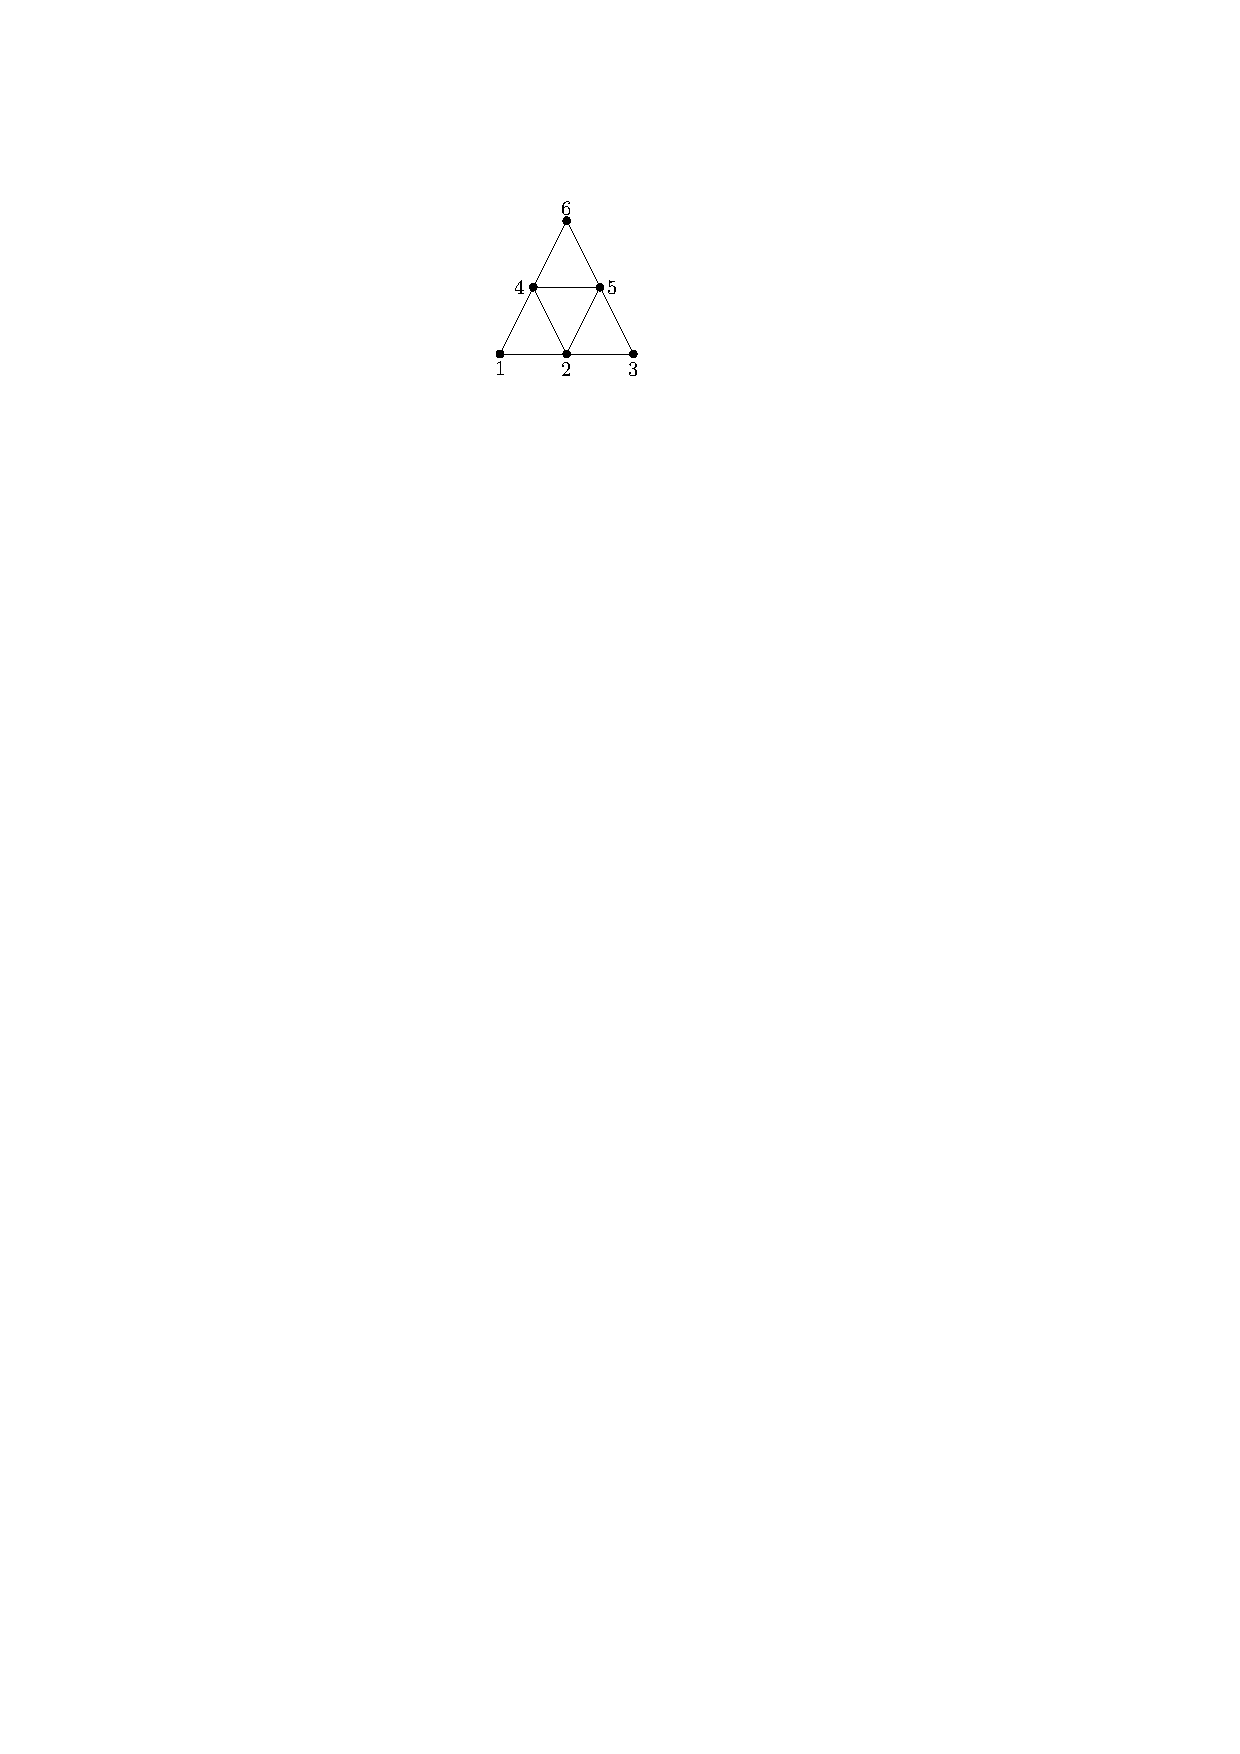
\includegraphics[page=1,width=0.5\linewidth]{graphics/preliminaries_drawing_models.pdf}
		\caption{}\label{im:drawing_models_a}
	\end{subfigure}
\begin{subfigure}{0.4\textwidth}
	\centering
	\includegraphics[page=2,width=\linewidth]{graphics/preliminaries_drawing_models.pdf}
	\caption{}\label{im:drawing_models_b}
\end{subfigure}
\begin{subfigure}{0.4\textwidth}
	\centering
	\includegraphics[page=3,width=\linewidth]{graphics/preliminaries_drawing_models.pdf}
	\caption{}\label{im:drawing_models_c}
\end{subfigure}
	\caption{\ref{im:drawing_models_a} is a straight-line drawing of a maximal outerplanar graph $G$, \ref{im:drawing_models_b} is a box drawing of $G$ and \ref{im:drawing_models_c} is a polyline drawing derived from \ref{im:drawing_models_b}}\label{im:drawing_models}
\end{figure}

\subsection{Graph Classes}
\subsubsection{Tree}
A graph $T$ is called \emph{tree} if and only if it is connected, acyclic and undirected \cite[P. 1172]{DBLP:cormen_intro_to_algorithms}.\\
% rooted
A tree is \emph{rooted} if one of its vertices is distinguished from the other ones, called the \emph{root}. Unless otherwise mentioned, it is assumed that every tree is rooted at the root vertex $r$. 

% path ancestor parent sibling
When considering a path $(r,v_1,...,v_k)$ from $r$ to any other vertex $v_k$, then, the following holds:
\begin{enumerate}
	\item Besides $w$, every vertex of this path is an \emph{ancestor} of $w$
	\item For an edge $(v_i,v_{i+1})$, $v_i$ is called the \emph{parent} of $v_{i+1}$, and $v_{i+1}$ is a child of $v_i$.
	\item The \emph{height} of the root $r$ is set to 0. For a vertex $v$ of $T$ it holds that its height is larger by one unit than its parent.
\end{enumerate}
% leaves, internal nodes
A vertex with no children is called a \emph{leaf}. Any vertex which is not a leaf is called an \emph{internal node}.
% level
A \emph{level} of $T$ consists of all vertices of the same height.
% height
The \emph{height} of $T$ is equal to the largest height of any vertex of $T$. \cite[P. 1176ff]{DBLP:cormen_intro_to_algorithms}
% complete k-ary tree
A \emph{$k$-ary tree} is a rooted tree in which for every vertex has at most $k$ children.
A \emph{complete $k$-ary tree} is a $k$-ary tree in which all leaves have the same height and all internal nodes have $k$ children.
\subsubsection{Outerplanar Graphs, Series Parallel Graphs and 2-Trees}
% outerplanar graph
An \emph{outerplanar graph} is a planar graph that can be drawn without crossing in a way so that all vertices are on the outer face. A \emph{maximal outerplanar graph} is an outerplanar graph to which it is not possible to add an edge without destroying the simplicity, planarity or outerplanarity property. 
% series parallel graph
A \emph{2-terminal series-parallel graph} with terminals $s,t$ is a recursively defined graph with one of the following three rules:
\begin{enumerate}
	\item An edge $(s,t)$ is a 2-terminal series-parallel graph
	\item If $G_i, i = 1,2$, is a 2-terminal series-parallel graph with terminals $s_i,t_i$, then in the serial composition $t_1$ is identified with $s_2$ to obtain a 2-terminal series-parallel graph with $s_1,t_2$ as terminals
	\item If $G_i, i=1,...,k$, is a 2-terminal series-parallel graph with terminals $s_i,t_i$, then in a parallel composition we identify all $s_i$ into one terminal $s$ and all $t_i$ into the other terminal $t$ and the result is a 2-terminal series-parallel graph with terminals $s,t$.
\end{enumerate}
A \emph{series-parallel graph}, \emph{SP-graph} in short, is a graph for which every biconnected component is a 2-terminal series-parallel graph. A SP-graph is \emph{maximal} if no edge can be further added while maintaining a SP-graph. \cite[P. 143ff]{Biedl_SP}\\
% 2-tree
A \emph{$k$-tree} is a recursively defined graph with at least $k+1$ vertices. If $n = k+1$, then the $k$-tree is the complete graph $K_{k+1}$. If $n>{k+1}$, start with a $K_{k+1}$ and every vertex added is adjacent to exactly $k$ adjacent neighbours. The class of \emph{2-trees} correspond to the class of maximal SP-graphs \cite[Page 2]{straight-line_2-trees}.
\subsection{Tools}
% SPQR Tree
\subsubsection{$SPQR$-Tree}
A \emph{cut vertex} in a graph $G$ is a vertex whose removal disconnects $G$. A \emph{separation pair} in $G$ is a pair of vertices whose removal disconnects $G$. A \emph{biconnected component} of $G$ is a maximal (in terms of vertices and edges) biconnected subgraph of $G$. If $G$ contains vertices $s,t$, then $G$ is \emph{$st$-biconnectable} if $G \cup \{s,t\}$ is biconnected. A \emph{split pair} of $G$ is either a separation pair or a pair of adjacent vertices of $G$. A \emph{maximal split component} of $G$ in regard to a split pair $\{u,v\}$ is either an edge $(u,v)$ or a maximal subgraph $G'$ of $G$ such that $G'$ contains $u$ and $v$ and $\{u,v\}$ is not a split pair of $G'$. A vertex $w$ aside from $u$ and $v$ belongs to exactly one maximal split component. A \emph{split component} of $\{u,v\}$ is defined as the union of any number of maximal split components of $\{u,v\}$. A split pair $\{u,v\}$ is \emph{maximal}, if there is no split pair $\{w,z\}$ in $G$ such that $\{u,v\}$ is contained in a split component of $\{w,z\}$.\\
The \emph{SPQR-Tree} $\mathcal{T}$ of $G$ is a recursively defined composition of $G$ with respect to its split pairs. $\mathcal{T}$ is a rooted tree with four types of nodes: $S,P,Q$ and $R$. Any node $\mu$ of $\mathcal{T}$ is related to a planar $uv$-biconnectible multigraph, the so-called \emph{skeleton} of $\mu$, denoted as $sk(\mu)$. $\mathcal{T}$ is recursively defined - Let $(s,t)$ be an edge of $G$, called the \emph{reference edge}. $\mathcal{T}$ is initialized with a $Q$ node $\phi$ as root, representing the edge $(s,t)$. The skeleton of $\phi$ consists of two parallel edges $(s,t)$. One is a \emph{real }edge, one is a \emph{virtual }edge.\\
After the initialization of $\mathcal{T}$ with an arbitrary reference edge, consider a node $\psi$ of $\mathcal{T}$, $G_\psi=\left(V(G),E(G)\setminus\left\{(s,t)\right\}\right)$ and a pair of vertices $\{u,v\}$ of $G_\psi$, called the \emph{poles} of $\psi$.

\begin{description}
	\item[Trivial case] If $G_\psi$ consists of a single edge $(u,v)$, then $\psi$ is a $Q$-node. In this thesis, this case will be denoted as $Q(u,v)$.
	\item[Series case] If $G_\psi$ is not a single edge and not biconnected, then $\psi$ is a $S$-node with at least one cut vertex $c$ between the path between $u$ and $v$. In this thesis, this case will be denoted as $S(u,c,v)$.
	\item[Parallel case] If $G_\psi$ is not a single edge, but biconnected with $\{u,v\}$ as a split pair of $G_\psi$, then $\psi$ is a $P$-node. In this thesis, this case will be denoted as $P(u,v)$.
	\item[Rigid case] If $G_\psi$ is not a single edge, biconnected with $\{u,v\}$ not being a split pair of $G_\psi$, then $\psi$ is a $R$-node. Due to the properties of the graph classes considered in this thesis, this case will not be covered in application and is not of further interest. 
\end{description}
\cite[P. 7-8]{SPQR-Tree}
% Tree decomposition / treewidth 
\subsubsection{Tree decomposition}
Let $G$ be a graph, $T$ a tree, and let $\mathcal{W} = \left(W_t\right)_{t\in T}$ be a family of vertex sets $W_t \subseteq V_G$ indexed by the vertices $t$ of $W$. The pair $(T,W)$ is called a \emph{tree decomposition} of $G$ if it satisfies the following three conditions:
\begin{enumerate}
	\item $V_G = \bigcup_{t\in T}W_t$
	\item For every edge $e\in E_G$ there exists a $t\in T$ such that both ends of $e$ lie in $W_t$
	\item For all $v\in V$, there exists a connected subtree $T'$ in $T$ such that $v \in W_{t'}, t' \in V_{T'}$
\end{enumerate}
\cite[P. 319]{Diestel_GraphTheory}
\\
The \emph{width} of a tree decomposition is defined as 
\begin{align}
	tw((T,W)) = \max\{ |W_t|,t\in V_T \} -1
\end{align}
The \emph{treewidth} of a graph is the least width of any tree decomposition of $G$ \cite[P. 321]{Diestel_GraphTheory}. A graph with a treewidth bound by $k$ is a $k$-tree \cite[P. 5]{k-tree_bounded-treewidth}.

\section{Initial Situation}\label{section:initial_situation}

\subsection{The Fixed Edge-Length Planar Realization Problem}

The \emph{Fixed Edge-Length Planar Realization Problem}, \emph{FEPR} problem in short, asks whether there exists a planar straight-line drawing of a given graph where the euclidian length of an edge is given by a function $\lambda: E(G) \to \mathbb{R}^+$.
\\
It was shown, that the \emph{FEPR} problem is generally \NP-hard for triconnected graphs with unit lengths as well as biconnected graphs with unit lengths, with $\lambda$ as a constant function. \cite[P. 2]{straight-line_2-trees}

\subsection{Formalization Of The Problem}
\subsubsection{The edge-length ratio}
Let $\Gamma_G$ be a given planar polyline drawing. The length of an edge is defined as the sum of $k+1$ line segments, induced by $k$ bends. $l_{\max}$ is the length of the longest edge in $\Gamma_G$, $l_{\min}$ is the minimal Euclidian distance between two adjacent vertices in $\Gamma_G$. Then, the edge-length ratio $r$ of $\Gamma_G$ is defined as:
\begin{align}
	r_{\Gamma_G} = \frac{l_{\max}}{l_{\min}} 
\end{align}
It trivially holds, that $r\geq1$, since the length of every polyline with at least one bend between two vertices is naturally longer than their respective Euclidian distance. $r$ is said to be \emph{optimal} if $r=1$. Then, all the edges in a drawing are straight-lines and of the same length. This corresponds to the \emph{FEPR} problem with $\lambda$ being a constant function.
\subsubsection{Upper bound of the ratio}
There exist multiple straight-line drawing algorithms which produce a drawing for a planar graph in area $\mathcal{O}(n)\times\mathcal{O}(n)$. Prominent examples are the Shift Method by Fraysseix, Pach and Pollack \cite [P. 202ff]{Planar_straight_line_drawing_algorithms} and Schnyder drawings \cite[P. 3]{Schnyder_drawings}.\\
The area consumption of a straight-line drawing directly induces the bounds for the ratio. Let $k\times k$ be the area consumption of a bounding square $\Gamma_G$ is drawn on, $k\in \mathcal{O}(n)$. The maximal length of a straight-line is then bound by $\sqrt{2}k$, from one corner of the grid to the diagonal opposing one, while $l_{\min}$ might value 1 \UL. The ratio therefore values $\sqrt{2}k \in \mathcal{O}(n)$ in the worst case.\\
This automatically gives an upper bound for any poly-line drawing $\Omega_G$ since a straight-line drawing can be seen as a polyline drawing with zero bends. Including bends in a straight-line drawing enables the possibility to reposition vertices in order to maximize the Euclidian distances.

% 2-trees state of the art

\subsection{On the edge-length ratio of 2-trees}

The class of $2$-trees is of particular interest in this thesis due to their balance in restricted properties on the one hand, and having non-trivial approaches and results for general problems on the other hand. $2$-trees are biconnected, but not triconnected. This property implies a high amount of possible embeddings for a given $2$-tree $G$, since parallel subgraphs can be permuted and flipped. Therefore, finding drawings with an optimization regarding a specific problem require combinatorial and algorithmic approches. This effect is pointed out by previous results regarding the edge-length ratio. It was shown that the \emph{FEPR} problem is \NP-hard for straight-line drawings for 2-trees with up to four distinct edge lengths while it is solvable in linear time for uniform edge lengths \cite[P. 1]{straight-line_2-trees}.\\
Also, it was proven that the ratio of straight-line drawings of 2-trees is unbounded, meaning, that for a given constant $r$, there exists a sufficiently large 2-tree $G$ with $r_G > r$ over all its straight-line drawings. One result states that the ratio lies in the gap between the lower bound $\Omega(\log n)$ and the upper bound $\mathcal{O}(n^{0.695})$ \cite[P. 2]{edge-length-ratio-2tree}.

% symposium challenge

\subsection{The Symposium Challenge}

The \emph{Live Challenge} takes place during the Graph Drawing Symposium in 2022. During one hour, teams will compete either manually or automatically with their own tools and implementation. The goal is to optimize the ratio for given graphs on a fixed grid. The team with the highest score achieved regarding the edge-length ratio wins. For teams participating with their own tools, an embedding might not be given with the input. For participants working manually, an embedding is already given beforehand.
\\
For the automatic section of the Live Challenge, the input consists of a JSON file with the following entries:
\begin{description}
	\item[nodes] Every node has an unique ID value between 0 and the amount of nodes - 1, a value for the $x$ and $y$ coordinate each, delimited by the width and height
	\item[edges] Every edge has an ID for source and destination each and an optional list of bend points, specified in $x$ and $y$ coordinate
	\item[width (optional)] The maximum $x$-coordinate of the grid. If unspecified, the width is set to 1,000,000.
	\item[height (optional)] The maximum $y$ coordinate of the grid. If unspecified, the height is set to 1,000,000.
	\item[bends] The maximum number of bends allowed per edge
\end{description}
The results of the optimization are also JSON files. The planarity of the graph shall be preserved and the ratio minimized by relocation of the nodes and using suitable bend points.
\bigskip
While the Live Challenge during the Graph Drawing Symposium addresses the practical aspects regarding the task of optimization, this thesis concerns approaches to guarantee an asymptotic behaviour of the ratio for certain graph classes. The grid 
% TODO difference between the practical aspect and the theoretical bounds
% TODO neues beispiel

\subsubsection{A small example}

This example will illustrate the issue of optimizing a drawing with respect to its edge-length ratio. 
 
% TODO example: only serial, only parallel?

%\begin{figure}[H]
%	\centering
%	\begin{subfigure}{0.6\linewidth}
%		\centering
%		\includegraphics[width=0.7\textwidth,page=1]{drawings/small_example.pdf}
%	\end{subfigure}
%	\caption{There is no grid point for an optimal drawing without any bends}
%\end{figure}
%But, when introducing one bend per edge, there exists a drawing with an optimal ratio. 
%\begin{figure}[H]
%	\centering
%	\begin{subfigure}{0.6\linewidth}
%		\centering
%		\includegraphics[width=0.7\textwidth,page=2]{drawings/small_example.pdf}
%	\end{subfigure}
%	\caption{With one bend, $K_3$ admits an optimal drawing}
%\end{figure}
\section{$k$-ary Trees}

\section{Maximal Outerplanar Graphs}

This thesis addresses two main approaches of ratio minimization for drawings of series-parallel graphs. Maximal series-parallel graphs correspond to the class of 2-trees \cite[P. 2]{straight-line_2-trees} and are a suitable class of interest for fundamental research since any 2-tree is biconnected, but not triconnected and inherits a constant treewidth. Furthermore, any maximal outerplanar graph is a 2-tree, therefore the class of maximal outerplanar graphs is a strict subclass of the 2-trees.\\
At first, the approaches will address the maximal outerplanar graphs since maximal outerplanar graphs are a subclass of maximal SP-graphs. After the analysis regarding the properties of the resulting drawings it will be discussed whether the approach will be suitable to be extended for 2-trees. This section will present two polyline drawing algorithms. The first drawing algorithm takes advantage of the already existing drawing algorithm \ref{al:k-ary_trees} for $k$-ary trees, since the weak dual graph of a maximal outerplanar graph inheits a tree structure. The second drawing algorithm for outerplanar graphs will be suited to be extended for $2$-trees, since every maximal SP-graph contains a maximal outerplanar graph as a subgraph.

\subsection{Properties Of Maximal Outerplanar Graphs}
\begin{lemma}
	A maximal outerplanar graph $G$ inherits triangles as inner faces, except for the outerface.
\end{lemma}
\begin{lemma}\label{l:outerplanar-dual-tree-degree-3}
	The \emph{weak dual graph} $G^*$ of a maximal outerplanar graph $G$ is a simple tree with maximum degree 3 for any vertex.
\end{lemma}
\begin{proof}
	The weak dual graph $G^*$ is connected since $G$ is maximal outerplanar. Suppose, that $G^*$ contains a cycle $\mathcal{C}$. Then, there exists a vertex in $G$ which is enclosed from the outerface by faces according to $\mathcal{C}$ in $G^*$ and $G$ is not outerplanar. This implies that $G^*$ must be acyclic and considering the connectedness, $G^*$ is a tree. Since any face $f$ is a triangle, the degree of $v_f$ in $G^*$ values at most three. The simplicity is derived from the maximal outerplanarity property. If there were multiple edges between vertex $v_f$ and $v_{f'}$ in $G^*$, then there would be at least one vertex in $G$ which does not lie on the outerface.
\end{proof}
\begin{lemma}
	Let $G$ be a maximal outerplanar graph with $n$ vertices and $G^*$ the dual graph excluding the outerface, a rooted tree with degree up to three for every vertex $v_f$. Then, the height of $G^*$ ranges between $\Omega(\log n)$ and $\mathcal{O}(n)$.
\end{lemma}
\begin{proof}
	Since $G$ is a planar graph, it contains $\mathcal{O}(n)$ faces. The rooted tree $G^*$ inherits the following property:
	\begin{enumerate}
		\item The root has at most three children
		\item The subtrees rooted at the children of the root are binary trees
	\end{enumerate}
	Placing $\mathcal{O}(n)$ vertices in three binary trees connected to a root vertex results in a height of at least $\Omega(\log n)$ due to the $k$-ary tree height property from Lemma \ref{l:k-ary-tree_log_height}. In the worst case, $G^*$ will be a chain of vertices, therefore a rooted tree with height $\mathcal{O}(n)$.
\end{proof}

\begin{lemma}
	A maximal outerplanar graph $G$ can be extended to a maximal outerplanar supergraph $G^+$.\label{l:outerplanar-supergraph}
\end{lemma}
\begin{proof}
	The vertex insertion works analougously to the recursive definition of a 2-tree. A new vertex can be added to $G$ by adding a new vertex $v_f$ in the dual graph $G^*$ so that the degree of $G^*$ is still at most 3. The newly created face $f$ must lie on the outerface and must be a triangle. Otherwise, the outerplanarity property is destroyed. 
\end{proof}

% One Bend, maximal complete outerplanar graph
\begin{observation}
	Let $G$ be a maximal outerplanar graph $G$ with a straight-line drawing $\Gamma_G$ and a ratio $r_G$. When $G$ is extended to a maximal outerplanar supergraph $G^+$, the ratio $r_{G^+}$ increases regarding $\Gamma_{G^+}$ based on $\Gamma_G$.\label{ob:area_leads_to_ratio_increase}
\end{observation}
When $G^*$ inherits a height of $\mathcal{O}(\log n)$, a new problem for a drawing emerges. When starting drawing the root of $G^*$, new vertices are added in all directions, enclosing more and more area along the iterative drawing, as illustrated in the following figures:
	\begin{figure}[H]
	\centering
	\begin{subfigure}{0.5\textwidth}
		\centering
		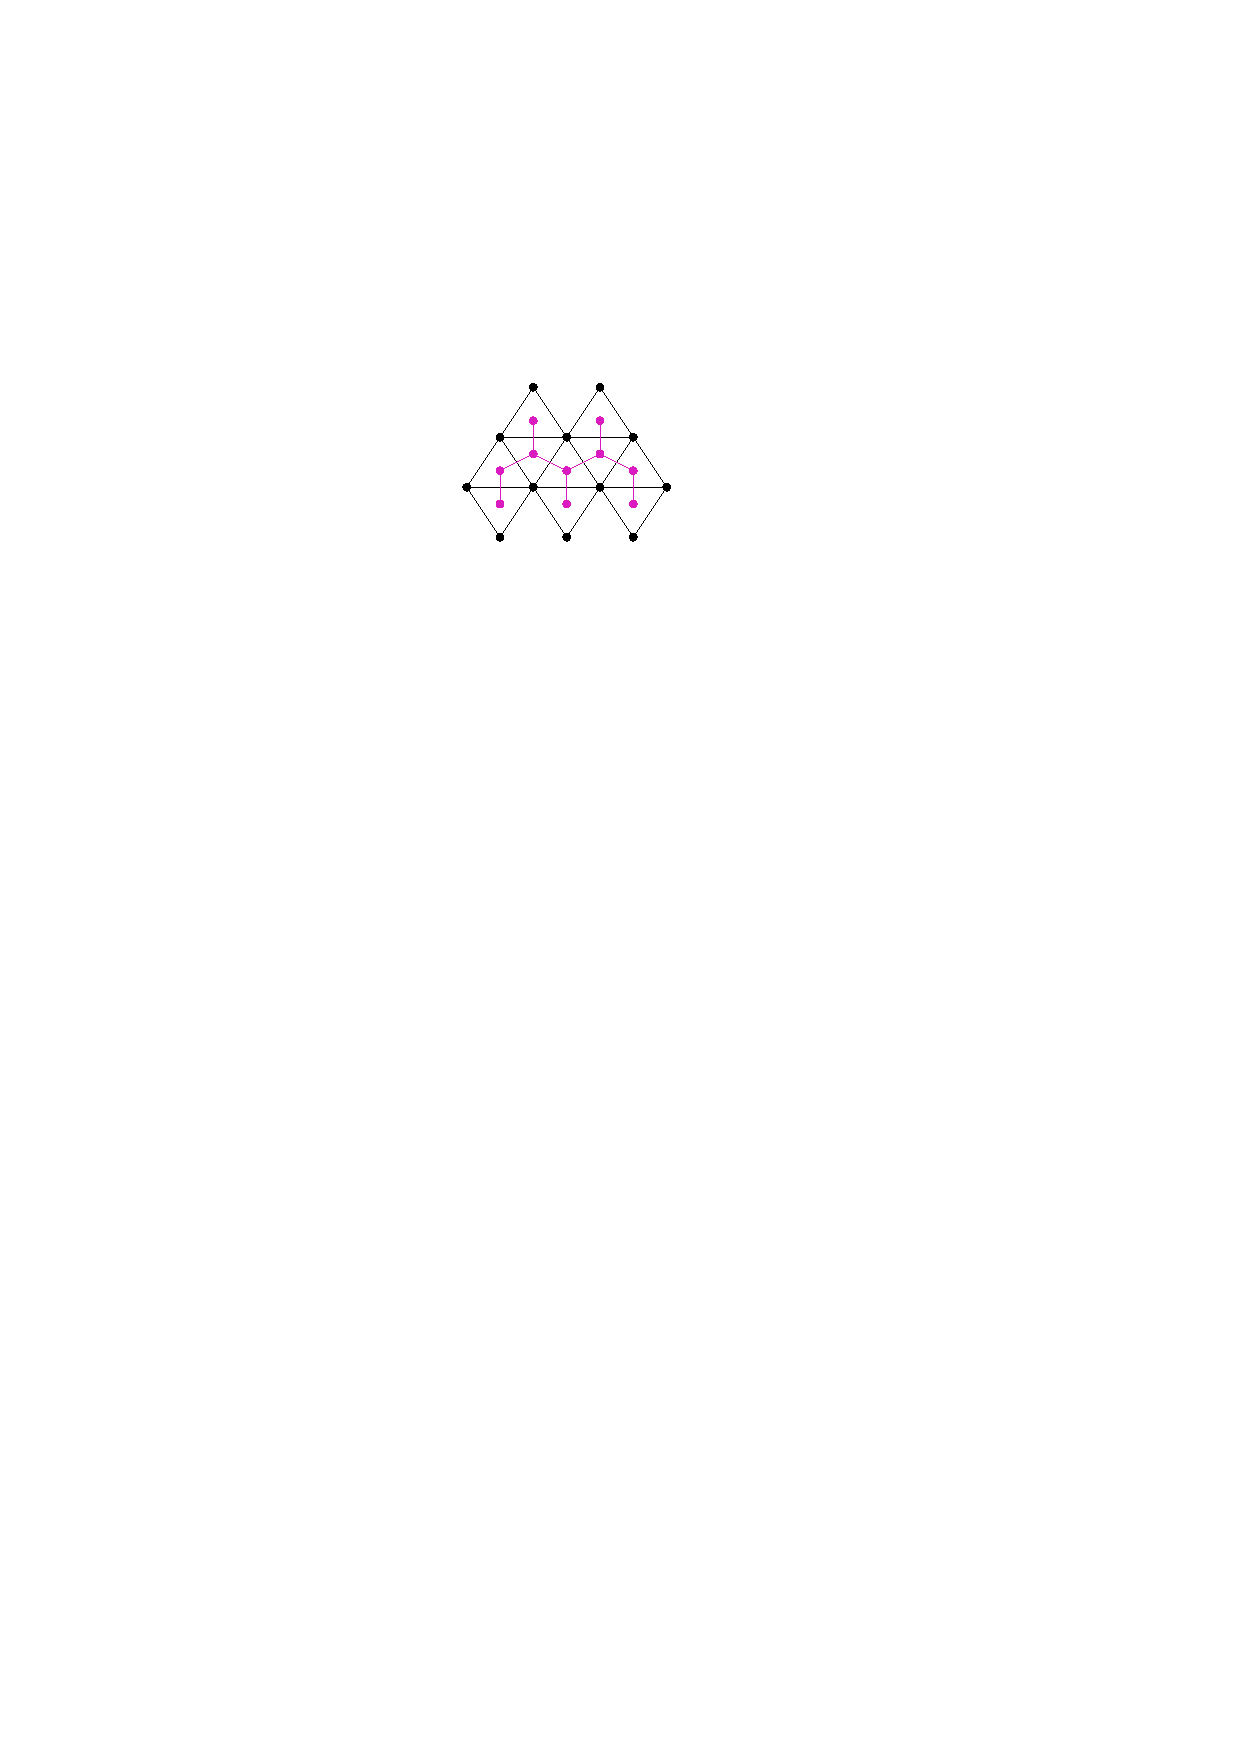
\includegraphics[page=1,width=0.7\linewidth]{graphics/maximal_outerplanar_extension_ratio.pdf}
		\caption{A straight-line drawing of a maximal outerplanar graph $G$ with its weak dual graph magenta-colored. The ratio is optimal}
	\end{subfigure}
	\begin{subfigure}{0.5\textwidth}
		\centering
		\includegraphics[page=2,width=0.7\linewidth]{graphics/maximal_outerplanar_extension_ratio.pdf}
		\caption{Extending $G$ results in a ratio increase due to area restrictions, colored in orange}
	\end{subfigure}
	\caption{Illustration of area restriction for dense maximal outerplanar graphs}
\end{figure}
This results in short euclidian distances relative to the longest edge, increasing the ratio.\\

\subsection{Drawing Algorithm For Complete Outerplanar Graphs With One Bend}
The first approach of a drawing algorithm addresses a ratio optimization for dense outerplanar graphs. These class of maximal outerplanar graphs are described with help of properties regarding the weak dual graph in the following way.
\begin{definition}\label{def:complete_maximal_outerplanar}
	A maximal outerplanar graph is called \emph{complete} if its weak dual graph $G^*$ fulfills these properties:
	\begin{enumerate}
		\item The root vertex has exactly three children
		\item Every other inner node has exactly two children. In other words, the subtrees adjacent to the root vertex are complete binary trees of height $h-1$
	\end{enumerate}
\end{definition}
A given maximal outerplanar graph can be drawn by using a drawing algorithm for its weak dual graph. In section \ref{s:k-ary_trees}, the $k$-ary tree drawing algorithm produces a straight-line drawing in $\mathcal{O}(n^2 \log n)$ area with a ratio of $1+\varepsilon,\varepsilon>0$. The drawing algorithm \ref{al:k-ary_trees} can be used with a minor modification to draw the weak dual graph of any complete maximal outerplanar graph $G$, since $G^*$ is a subtree of a $3$-ary tree with the same height.\\

\begin{algorithm}[H]
	\KwIn{A complete maximal outerplanar graph $G$}
	\KwOut{Straight-line drawing $\Gamma_{G^*}$ with nearly optimal ratio}
	\caption{\texttt{DrawOuterWeakDual($G$)}}\label{al:drawouterweakdual}
	$G^* \gets$ weak dual graph of $G$ with minimal height\\
	$h \gets$ \texttt{height($G^*$)}\\
	\texttt{root} $\gets$ $G^*$.\texttt{root}\\
	\texttt{Draw(root)}\\
	\texttt{Draw\_$3$-ary\_Children(\texttt{root},$3^h$,1)}\\
	\For{\texttt{$v \in$ root.children}}{
		\texttt{Draw\_$2$-ary\_Children($v$,$2^{h-1}$,$h-1$)}
	}
	\Return $\Gamma$
\end{algorithm}

Algorithm \ref{al:drawouterweakdual} produces a nearly optimal straight-line drawing for the weak dual graph of a complete outerplanar graph $G$. The resulting drawing $\Gamma_{G^*}$ provides assistance to draw the complete outerplanar graph $G$. Every vertex of $\Gamma_{G^*}$ serves as an anchor point for the drawing of its corresponding face in $G$.\\
Starting at the root of $G^*$, a triangle is drawn around the root in a way, that each edge of $G^*$ from the root to its three children crosses exactly one edge of the corresponding triangle face in $G$. The vertices for the triangle are placed as follows. The first vertex lies above the already drawn root with an euclidian distance to the root sufficiently high in order to preserve planarity for the remaining drawing. The other two vertices are placed inbetween the two triangles defined by the root, its $\{\text{left, right}\}$ and middle children.\\
In order to guarantee a valid vertex and bend placement at every inner node $v^*$, the drawing is stretched horizontally and vertically by a factor of three.\\
Then, the drawing algorithm iterates over the height of $G^*$. For every vertex $v^*$ of height $i\in \{1,...,h\}$ in $G^*$, two bend points are placed 1 \UL left and right from $\Gamma_{G^*}(v^*)$, and the new vertex $v$ is placed 1 \UL below from $\Gamma_{G^*}(v^*)$.\\
$v^*$ is adjacent to an edge $e^*$ defined in $G^*$ that is crossing exactly one edge $e = (v_1,v_2)$ of $G$. This crossing corresponds to the vertices defining the new face, $\{v, v_1, v_2\}$. Since $G^*$ consists of three complete binary subtrees connected to the root, using the bends to draw the new face will preserve planarity since the coordinate of every inner node inherits its unique $x$ value by construction of algorithm \ref{al:complete_k-ary_tree}.
This drawing approach is summarized in the following algorithm.\\
\begin{algorithm}[H]
	\KwIn{Complete outerplanar graph $G$}
	\KwOut{Polyline drawing $\Gamma_G$ with one bend per edge and ratio $\mathcal{O}(\log n)$}
	\caption{\texttt{DrawCompleteOuterplanar($G$)}}\label{al:complete_outerplanar}\label{algo:complete_outerplanar_graph_dual}
	$\Gamma \gets $ \texttt{DrawOuterWeakDual($G$)}\\
	$h \gets$ \texttt{height($G^*$)}\\
	\For{$v^* \in G^*$}{
		$x(v^*) \gets 3\cdot x(v^*)$
	}
	\tcc{Draw the triangle face around the root of ${G^*}$}
	$root \gets$ $\Gamma(G^*.\texttt{root})$\\
	$l \gets$ $\Gamma(G^*.\texttt{root.leftChild})$\\
	$m \gets$ $\Gamma(G^*.\texttt{root.middleChild})$\\
	$r \gets$ $\Gamma(G^*.\texttt{root.rightChild})$\\
	$v_1 \gets$ $\Gamma$.\texttt{PlaceVertex($x(root),y(root)+h\cdot 3^h$)}\\
	$v_2 \gets$ $\Gamma$.\texttt{PlaceVertex($\frac{x(root)+x(l)+x(m)}{3},\frac{y(root)+y(l)+y(m)}{3}$)}\\
	$v_3 \gets$ $\Gamma$.\texttt{PlaceVertex($\frac{x(root)+x(m)+x(r)}{3},\frac{y(root)+y(m)+y(r )}{3}$)}\\
	$\Gamma$.\texttt{DrawLineSegment($v_1,v_2$)}\\
	$\Gamma$.\texttt{DrawLineSegment($v_1,v_3$)}\\
	$\Gamma$.\texttt{DrawLineSegment($v_3,v_2$)}\\
	
	\tcc{Iterate over the height to draw the remaining vertices of $G$}
	\For{$i \in [1..h]$}{
		\For{$v^* \in G^*$ with height $i$}{
			$b_l \gets$ $\Gamma$.\texttt{PlaceBendPoint($x(v^*) - 1,y(v^*)$)}\\
			$b_r \gets$ $\Gamma$.\texttt{PlaceBendPoint($x(v^*) + 1,y(v^*)$)}\\
			$v \gets$ $\Gamma$.\texttt{PlaceVertex($x(v^*),y(v^*)-1$)}\\
			$e^* \gets (v^*,\texttt{parent}(v^*))$\\
			$e \gets (v_1, v_2)$ edge intersecting $e^*$
			\tcp{w.l.o.g. $v_1$ ordered left of $v_2$}
			$\Gamma.$\texttt{DrawLineSegment($v,b_l$)}\\
			$\Gamma.$\texttt{DrawLineSegment($b_l,v_1$)}\\
			$\Gamma.$\texttt{DrawLineSegment($v,b_r$)}\\
			$\Gamma.$\texttt{DrawLineSegment($b_r,v_2$)}
		}
	}
	$\Gamma$\texttt{.delete($G^*$)}\\
	\Return $\Gamma$
\end{algorithm}


\subsubsection{Analysis}

\begin{theorem}
	Every complete outerplanar graph $G$ admits a polyline drawing $\Gamma_G$ on $\mathcal{O}(n^2 \log n)$ area with one bend per edge, preserving outerplanarity. The drawing is constructed in linear time and the ratio lies in $\mathcal{O}(\log n)$.
\end{theorem}

\begin{proof}
	The triangle around the root of $G^*$ consists of a vertex $v_1$ placed atop of the root vertex with distance $h\cdot r^h$ and two vertices $v_2,v_3$ placed at the centroids of the triangles defined by $\{\texttt{root,root.leftChild,root.middleChild}\}$ and $\{\texttt{root,root.middleChild,root.rightChild}\}$. By construction it holds, that $v_2$ and $v_3$ partition three binary subtrees rooted at the children of the root of $G^*$ by their $x$ coordinate. The placement of the vertices $v_1,v_2$ and $v_3$ guarantee exactly one intersection between an edge of $G$ and an edge of $G^*$ in $\Gamma$.\\
	After stretching the drawing horizontally by a factor of three, there exist free grid points next to every vertex of $G^*$ which guarantees a grid point placement left and right of any vertex $v^*$. During the iteration over the height starting at height 1, every intersection between an edge of $G^*$ and $G$ refer to vertices on the outerface and a new face of $G$ is attached on the outerface, preserving the outerplanarity of the drawing.\\
	Since $v_1$ is placed with a distance of $h\cdot r^h$ atop of the root of $G^*$ and $v_2$ and $v_3$ partition the $x$ coordinate of the binary subtrees rooted at the children of the root of $G^*$, planarity is preserved.\\
	The resulting area bounds are asymptotically the same compared to a drawing of a $3$-ary tree since the width and the height are multiplied by a constant. The area consumption lies still in $\mathcal{O}(n^2 \log n)$.\\
	The construction of $G^*$ with minimal height lies in $\mathcal{O}(n)$ since there are $\mathcal{O}(n)$ faces for any maximal outerplanar graph. Drawing $G^*$ and $G$ lies in $\mathcal{O}(n)$. The runtime of this algorithm is therefore in linear time.\\
	The minimal euclidian distance values at least $2^h$ by construction of algorithm \ref{al:k-ary_trees} and lies in $\mathcal{O}(n)$. The length of the longest polyline spans the whole height of the drawing and lies in $\mathcal{O}(n \log n)$. The ratio lies therefore in $\mathcal{O}(\log n)$ since the height of $G^*$ lies in $\mathcal{O}(\log n)$.
\end{proof}
\subsubsection{Example Drawing}

	\begin{figure}[H]
	\centering
	\begin{subfigure}{\textwidth}
		\centering
		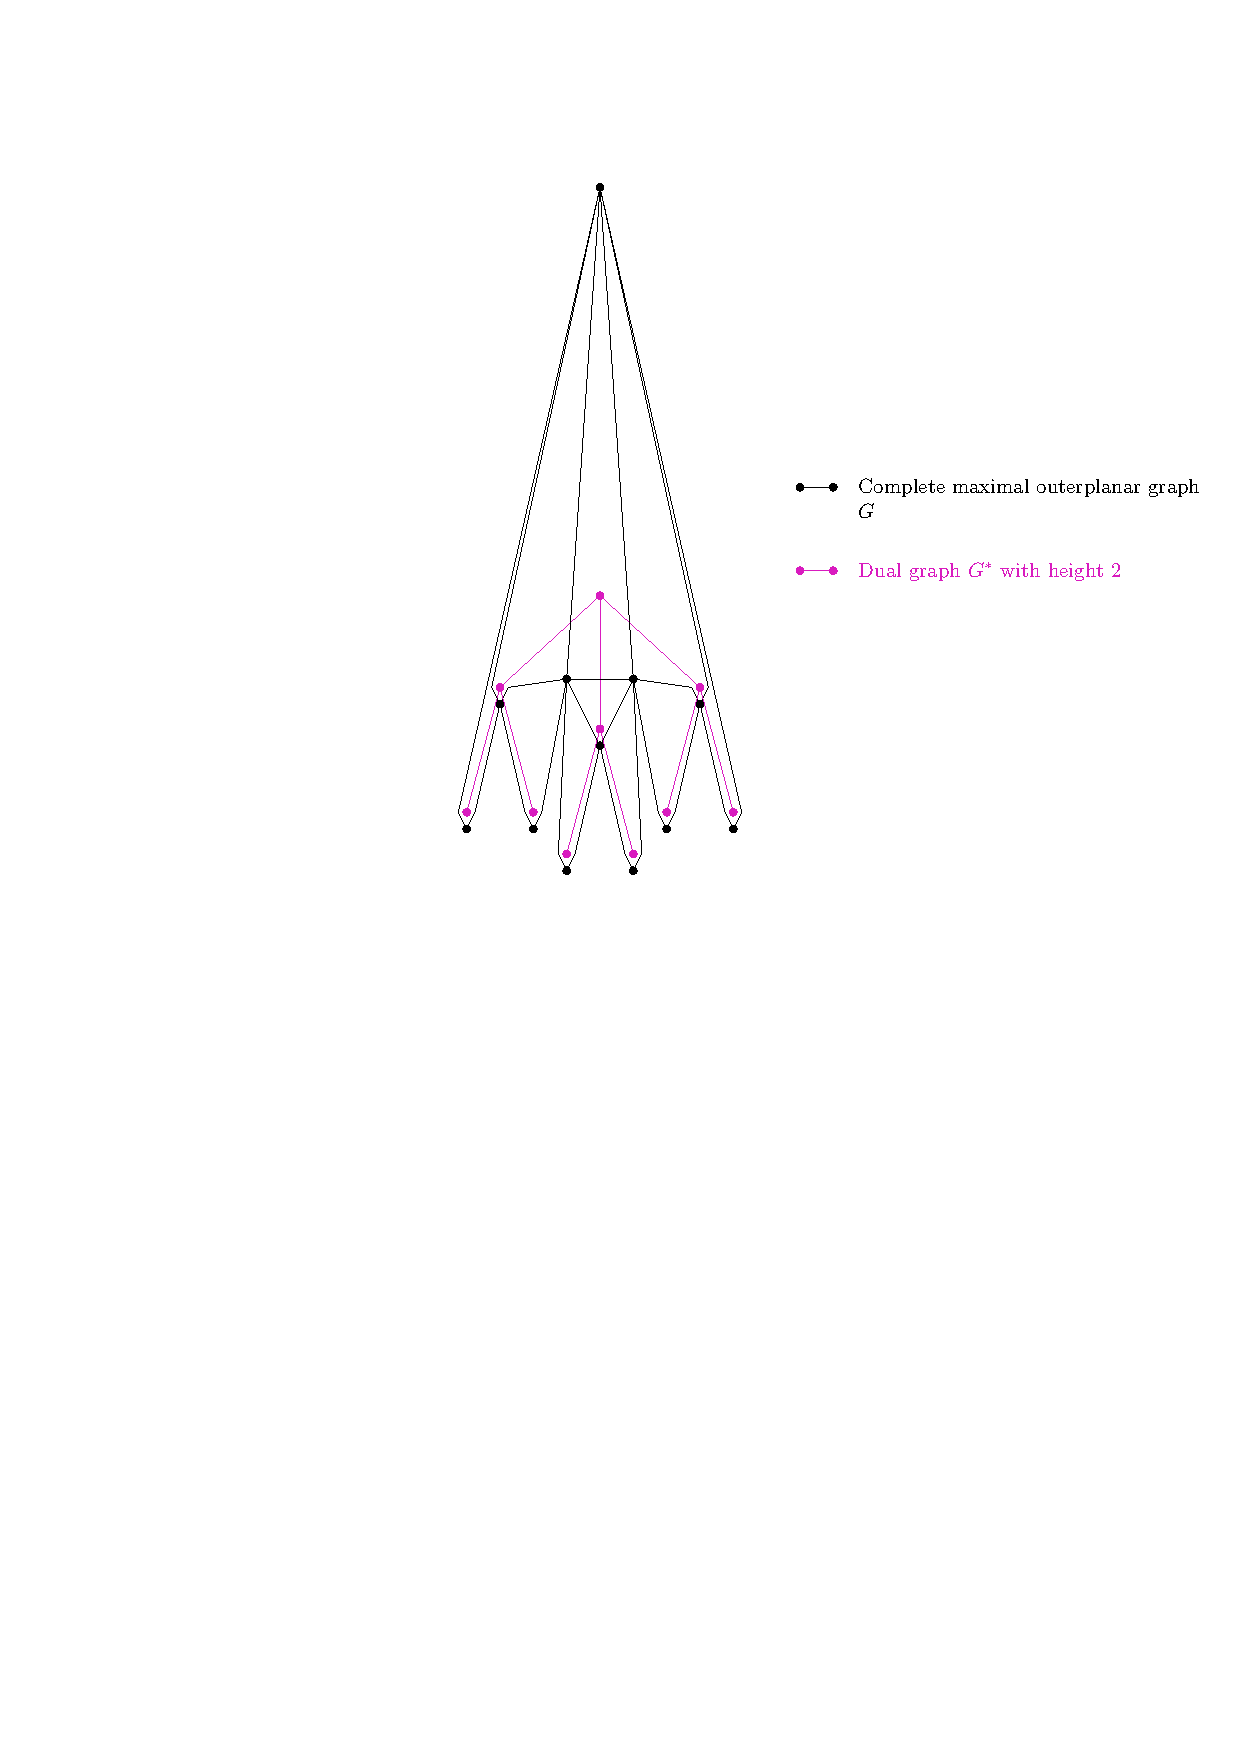
\includegraphics[page=1,width=0.7\linewidth]{graphics/complete_maximal_outerplanar_weak_dual_graph_example_drawing.pdf}
	\end{subfigure}
	\caption{Polyline drawing of a complete outerplanar graph $G$. The dual graph $G^*$ inherits a height of 2.}
\end{figure}


\subsubsection{Limitations}

As addressed by Observation \ref{ob:area_leads_to_ratio_increase}, this algorithm works fine for a complete maximal outerplanar graph $G$ since then, the height of $G^*$ is bound by $\mathcal{O}(\log n)$. On the other hand, when $G$ is a loose maximal outerplanar graph, a height of $G^*$ might be of linear size and therefore, the drawing algorithm is not improving the ratio contrary to a straight-line drawing. In addition, the drawing algorithm will only work for simple weak dual graphs. The weak dual graph of a maximal SP graph is a multigraph.
	\begin{figure}[H]
	\centering
	\begin{subfigure}{\textwidth}
		\centering
		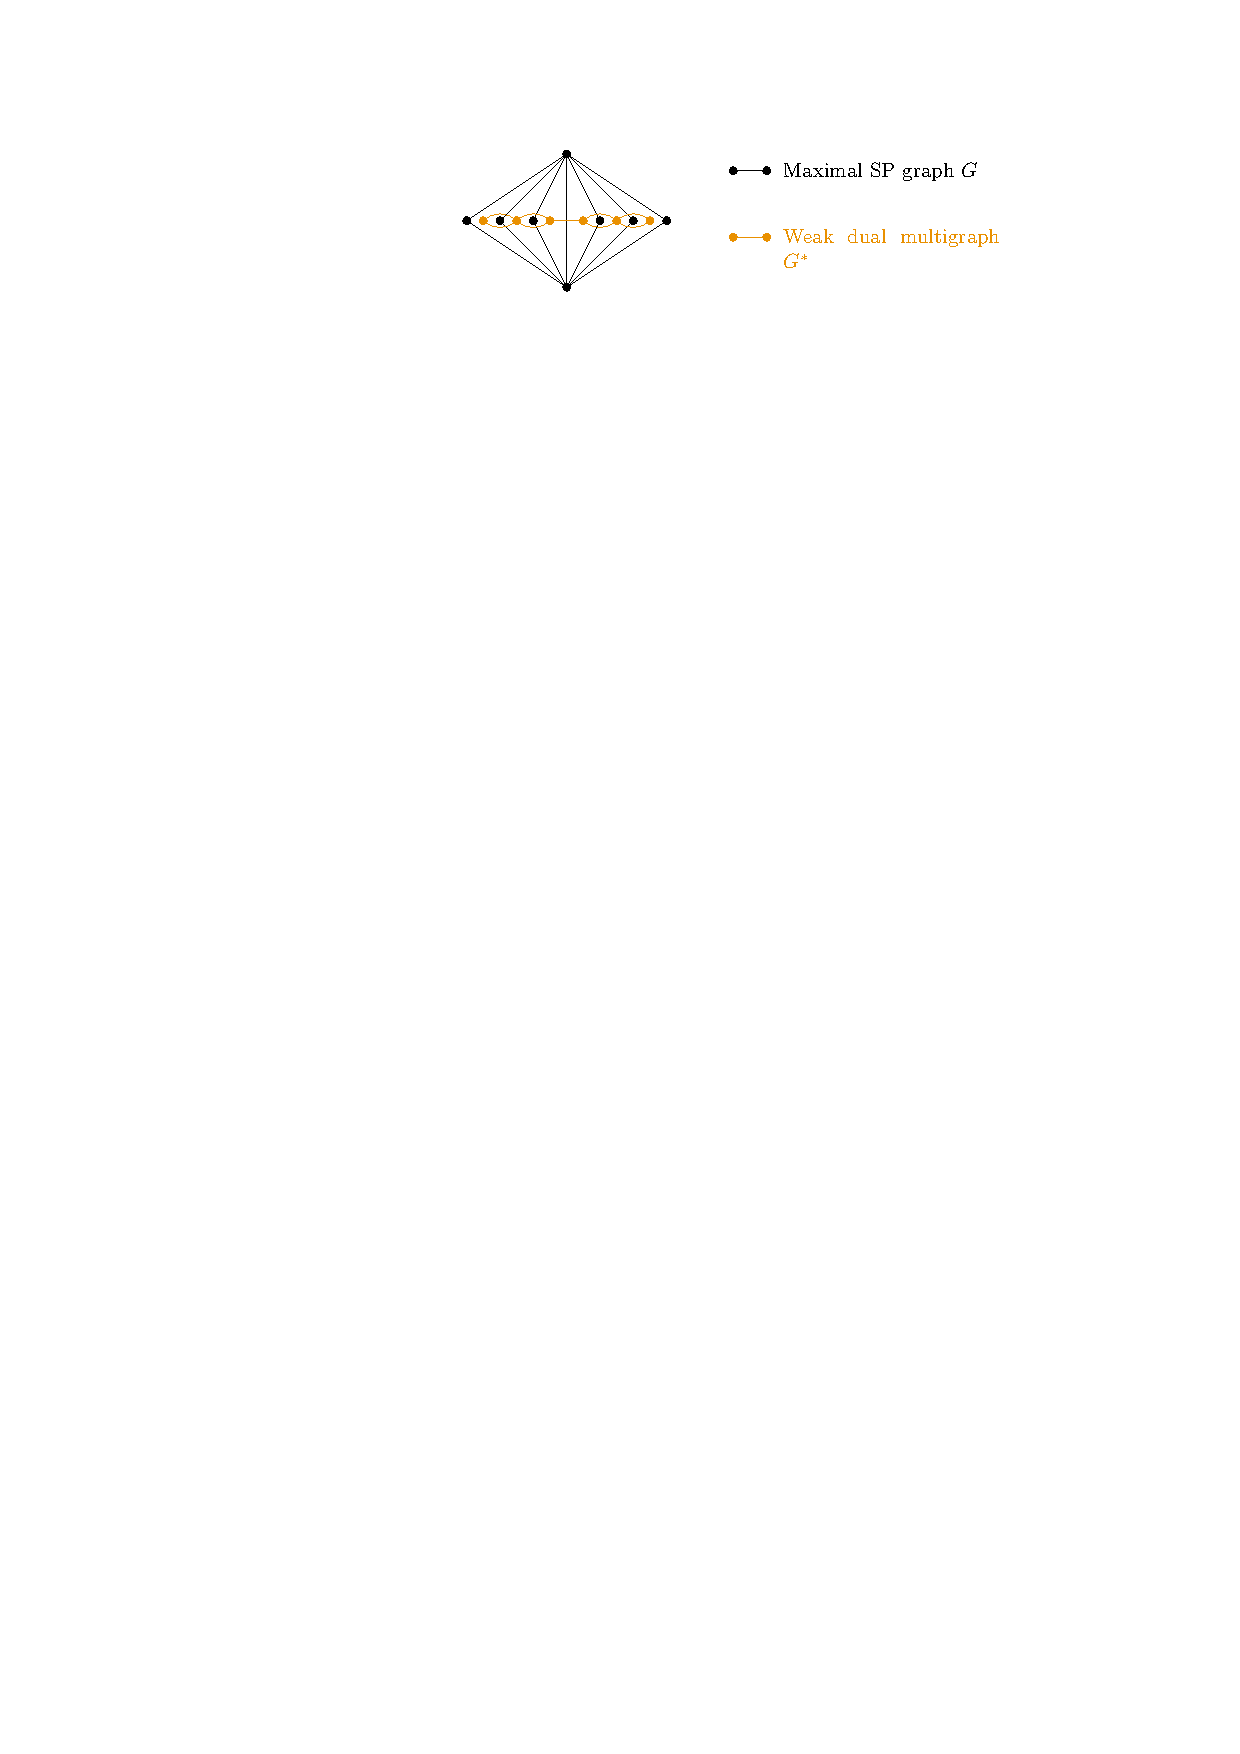
\includegraphics[page=1,width=0.6\linewidth]{graphics/maximal_sp_weak_dual.pdf}
	\end{subfigure}
	\caption{A maximal SP graph with its weak dual multigraph, colored in orange}
\end{figure}
The approach of drawing the weak dual graph at first followed by the outerplanar graph serves as an idea for a \emph{layered drawing}. The resulting drawings are valid layerings since the vertices of $G$ added on a fixed height of $G^*$ are not adjacent. As already observed, a layered drawing algorithm might guarantee a reasonable ratio by defining a minimal distance between two layers and therefore between two adjacent vertices. Since the weak dual graph is not suitable for 2-trees, the \emph{tree decomposition} of an SP-graph will serve as a guidance tool for the sequence of vertices drawn by a layering algorithm. The drawing algorithm will use the \emph{SPQR tree} derived from a tree decomposition.\\
When analyzing upper bounds for the ratio of a drawing for a maximal outerplanar graph $G'$, it is crucial to take a look at the tree structure of its tree decomposition. The following definition describes the difference of a $k$-ary tree $T$ to being a complete $k$-ary tree. This description of $k$-ary tree partitionings is very similar to a tree decomposition and will help during the analysis of a maximal outerplanar graph $G$ with its tree decomposition, since any tree decomposition is a $k$-ary tree.
\subsection{Partitioning A $k$-ary Tree In Complete $k$-ary Subtrees}
\begin{definition}
	A \emph{partitioning} $P = (\mathcal{P},\mathcal{W})$ of a $k$-ary tree $T$ is defined with the following properties:
	\begin{itemize}
		\item For every vertex $p$ in $\mathcal{P}$ there exists a bag $w$ in $\mathcal{W}$
		\item Every bag $w$ in $\mathcal{W}$ contains a complete $k$-ary subtree of $T$ and is non-empty
		\item If there exists an edge in $T$ between two complete subtrees described by $w_1$ and $w_2$ out of $\mathcal{W}$, then $p_1$ and $p_2$ share an edge in $\mathcal{P}$
		\item $\mathcal{P}$ is a rooted tree		
	\end{itemize}
	A \emph{partition} is a pair consisting of a vertex of $\mathcal{P}$ and its corresponding bag $\mathcal{W}$. A partitioning $P$ is \emph{minimal} if every other partitioning $P'$ of $T$ contains a higher amount of partitions.
\end{definition}
Let $T$ be a $k$-ary tree with $n$ vertices. Then, for a partitioning $P$ covering all the vertices of $T$, the following holds:
\begin{enumerate}
	\item The amount of partitions of size $\mathcal{O}(1)$ is bound by $\mathcal{O}(n)$
	\item The amount of partitions of size $\mathcal{O}(\log n)$ is bound by $\mathcal{O}\left(\frac{n}{\log n}\right)$
	\item The amount of partitions of size $\mathcal{O}(\sqrt{n})$ is bound by $\mathcal{O}(\sqrt{n})$
	\item The amount of partitions of size $\mathcal{O}(n)$ is bound by $\mathcal{O}(1)$
\end{enumerate}
Also, any combination of partitions are possible. Presuming that a partitioning covers $\mathcal{O}(n)$ vertices of a graph, any combination of multiple partitionings of constant amount is possible. For example, let $|V(G)| = 2n$. One chain of $\mathcal{O}(n)$ vertices followed by a complete $k$-ary tree with $n$ vertices results in a legitimate $k$-ary tree with height $\mathcal{O}(n)$. The minimal partitioning of this example consists of $\mathcal{O}(n)$ partitions in total.
	\begin{figure}[H]
	\centering
	\begin{subfigure}{\textwidth}
		\centering
		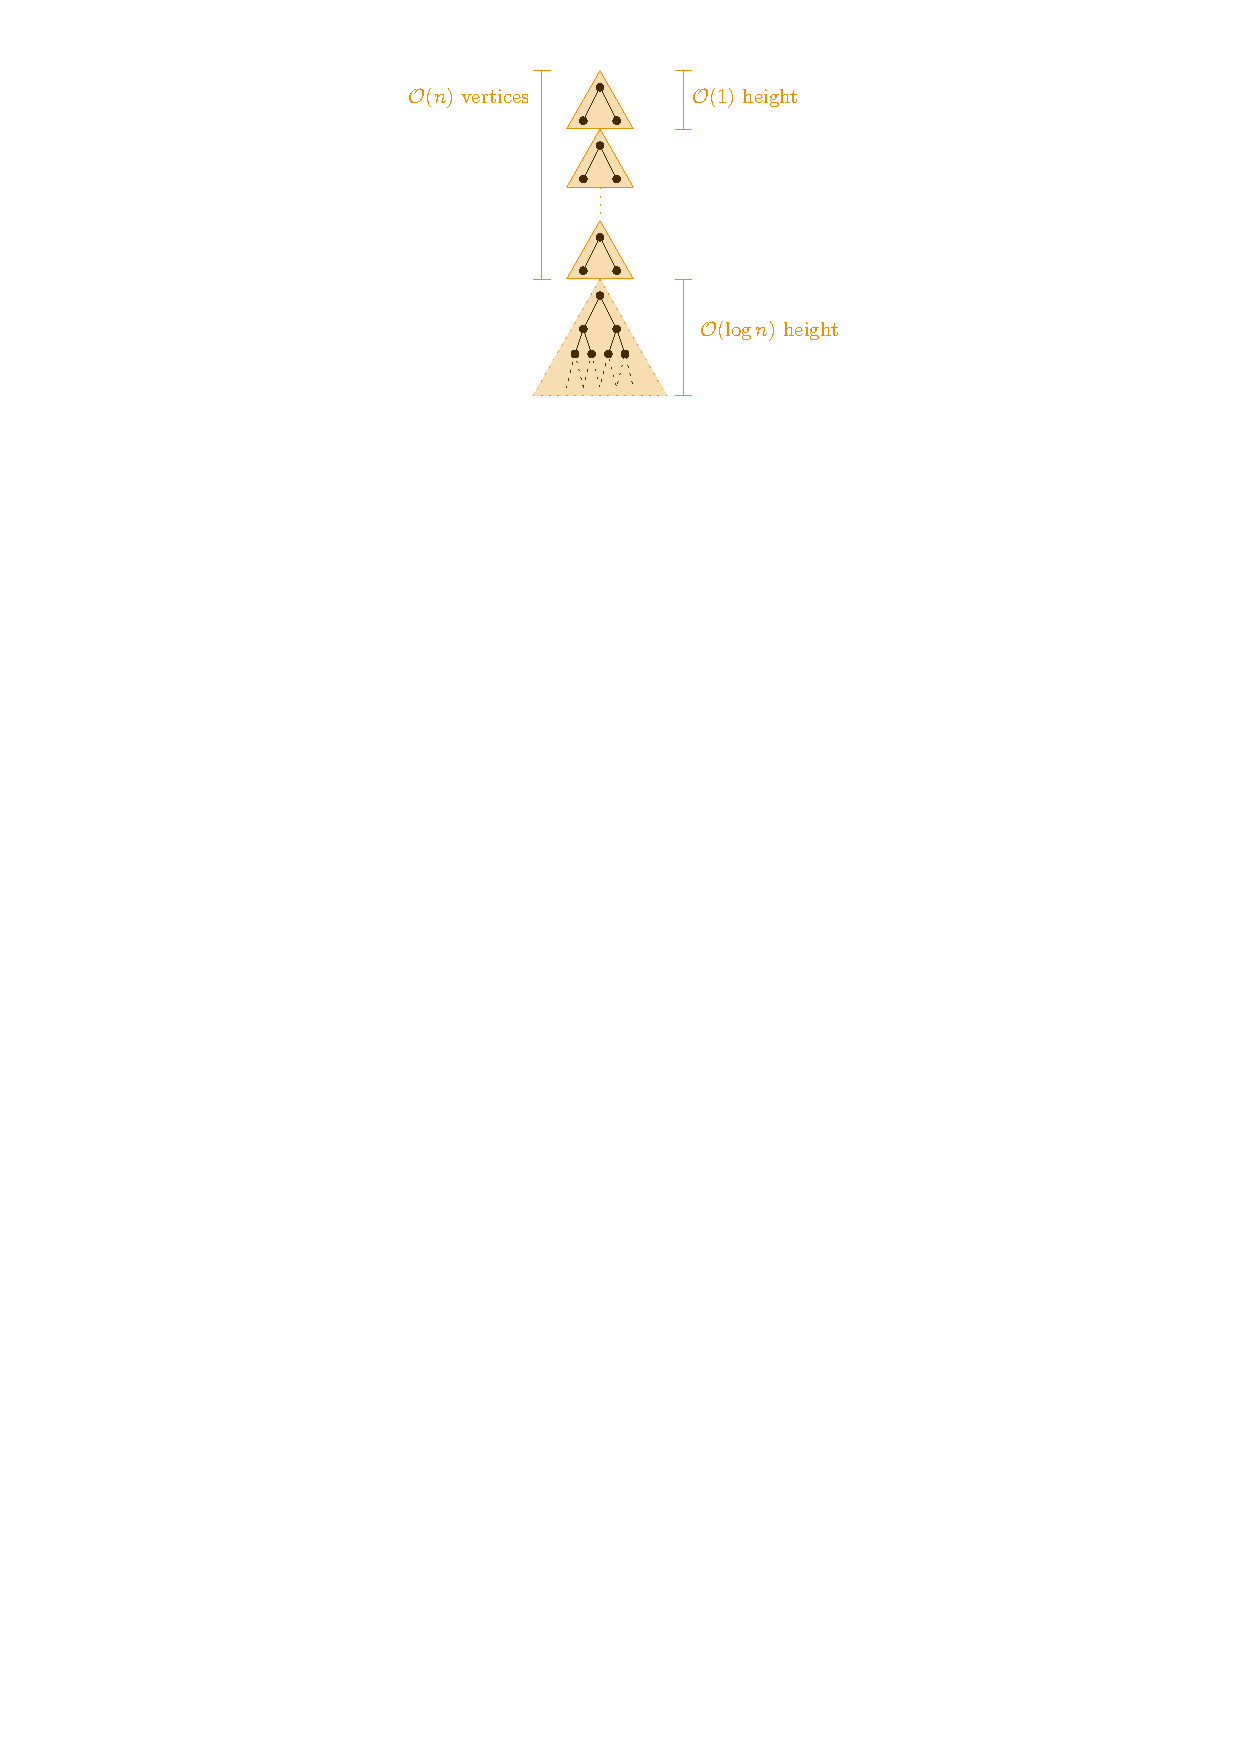
\includegraphics[page=1,width=0.7\linewidth]{graphics/k-ary_tree_partitioning_example.pdf}
	\end{subfigure}
	\caption{A $k$-ary tree of $\mathcal{O}(n)$ height partitioned in complete $k$-ary subtrees (in orange)}\label{im:partitioning_example}
\end{figure}


\begin{lemma}\label{l:partition_binary_tree_lower_upper_bounds}
	The height of $G$ interacts with the minimal partitioning $P$ of $G$ in the following way:
	\begin{enumerate}
		\item If $P$ consists of $\mathcal{O}(n)$ many partitions of constant size, the height of $G$ lies between $\Omega(\log n)$ and $\mathcal{O}(n)$
		\item If $P$ consists of $\mathcal{O}\left(\frac{n}{\log n}\right)$ partitions of size $\mathcal{O}(\log n)$, then the height of $G$ lies between $\Omega\left(\log\left(\frac{n}{\log n}\right)\cdot \log \log n \right)$ and $\mathcal{O}\left( n\right)$
		\item If $P$ consists of $\mathcal{O}(\sqrt{n})$ partitions of size $\mathcal{O}(\sqrt{n})$, then the height of $G$ lies between $\Omega(\log^2 n)$ and $\mathcal{O}(\sqrt{n}\log n)$
		\item if $P$ consists of a constant amount of partitions of size $\mathcal{O}(n)$, then the height is bound by $\mathcal{O}(\log n)$.
	\end{enumerate}
\end{lemma}
\begin{proof}
	Let $T$ be a $k$-ary tree and $P=(\mathcal{P},\mathcal{W})$ its minimal partitioning. Without loss of generality, it is presumed that all partitions of $P$ are of the same size. Since $\mathcal{P}$ is a tree, the following extremal cases for $\mathcal{P}$ are considered for the height of $T$:
	\begin{figure}[H]
		\centering
		\begin{subfigure}{0.6\textwidth}
			\centering
			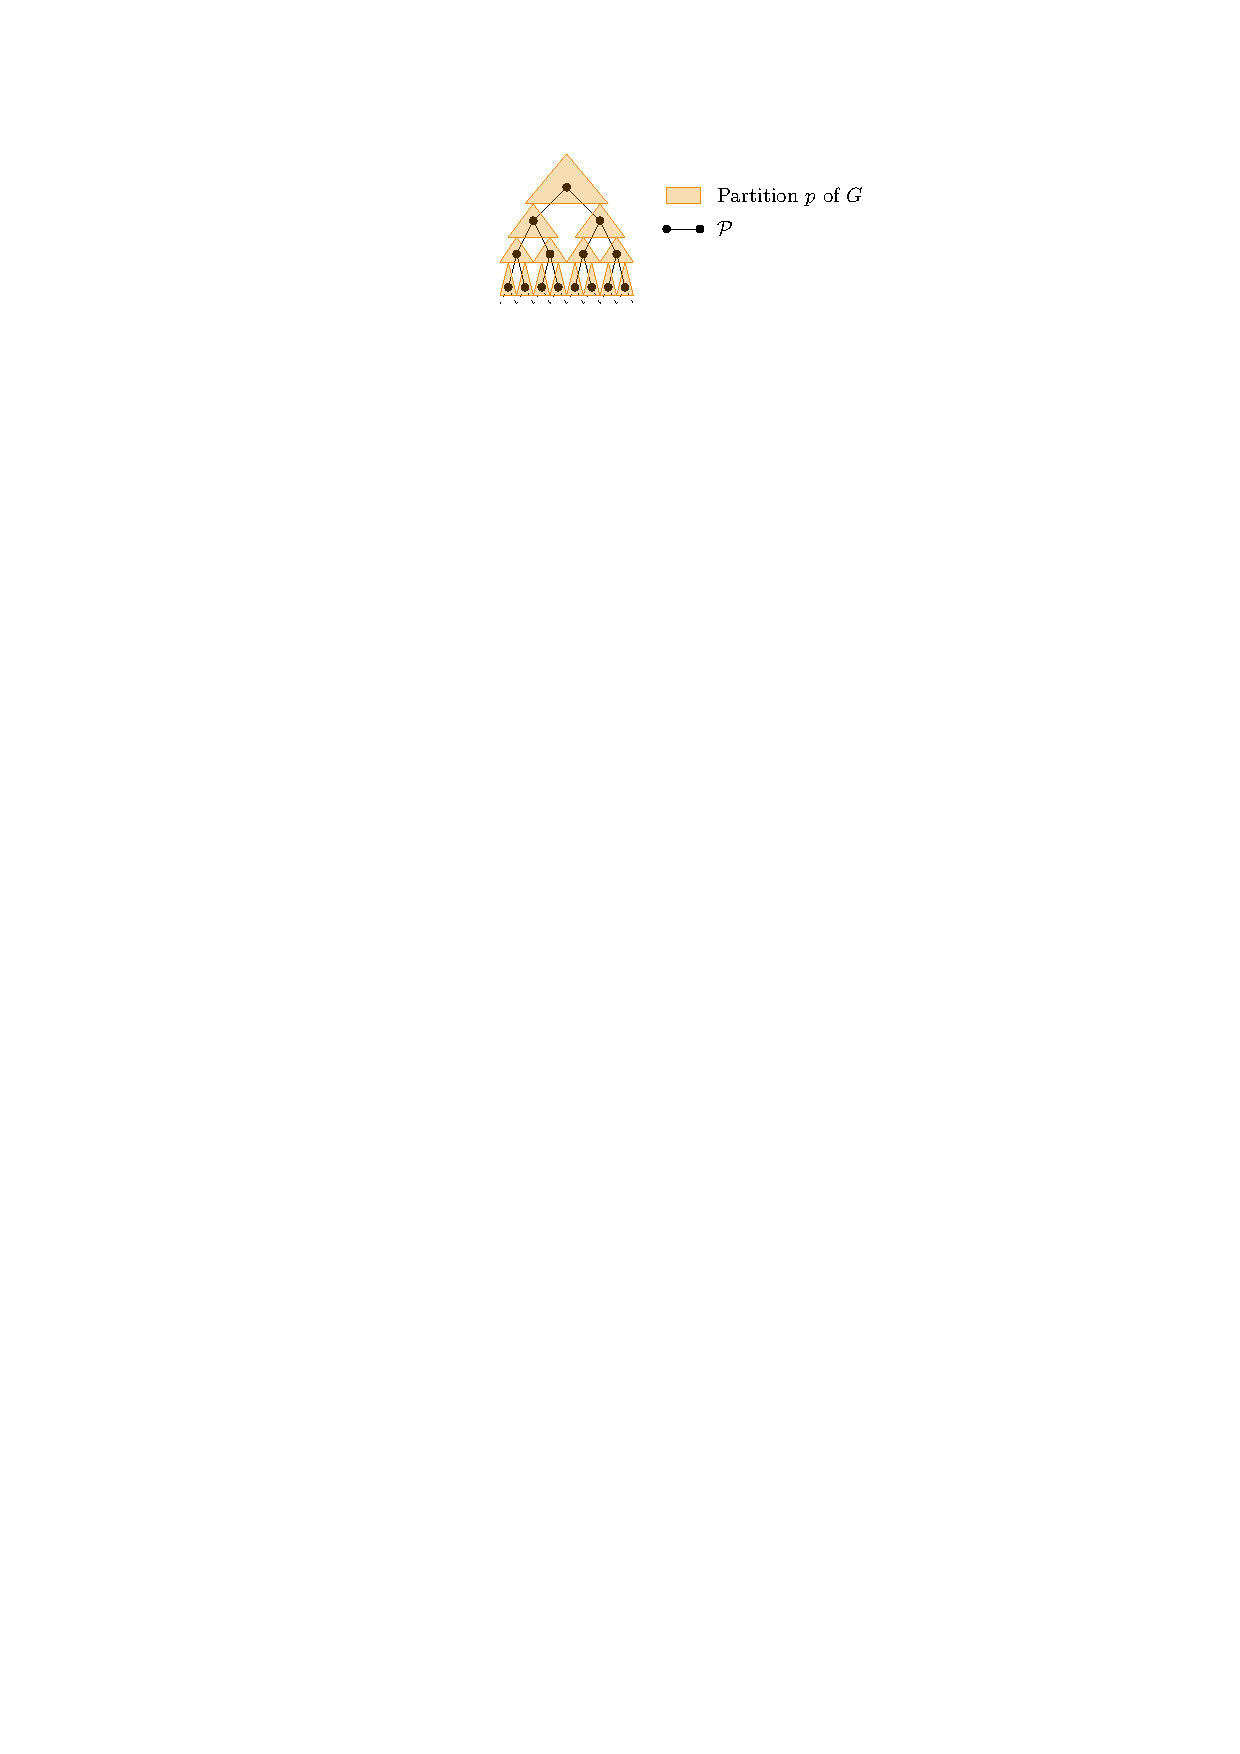
\includegraphics[page=1,width=\linewidth]{graphics/Partitioning_scheme.pdf}
			\caption{$\mathcal{P}$ represents a complete binary tree}\label{im:partitioning_binary}
		\end{subfigure}
		\begin{subfigure}{0.6\textwidth}
			\centering
			\includegraphics[page=2,width=\linewidth]{graphics/Partitioning_scheme.pdf}
			\caption{$\mathcal{P}$ represents a chain of vertices}\label{im:partitioning_chain}
		\end{subfigure}
		\caption{Extremal cases regarding the structure of $P$ of a partitioning $\mathcal{P}$}\label{im:partitioning_scheme}
	\end{figure}
	One extremal case covers $\mathcal{P}$ being a complete binary tree. By Lemma \ref{l:k-ary-tree_log_height}, for the height investigation of $G$ it suffices $\mathcal{P}$ to be binary since every complete $k$-ary tree has asymptotically the same height bound. The other extremal case covers a chain of vertices of $\mathcal{P}$. For case \ref{im:partitioning_binary}, $\mathcal{P}$ is a tree with height $\mathcal{O}(\log |\mathcal{P}|)$ and up to $\mathcal{O}(|\mathcal{P}|)$ height in case \ref{im:partitioning_chain}.
	\begin{enumerate}
		\item A complete $k$-ary tree of constant size inherits a constant height. With $|\mathcal{P}|\in \mathcal{O}(n)$, substituting every vertex of $\mathcal{P}$ with complete $k$-ary trees of constant height does not alter the height asymptotically and the height bounds are valid.
		\item A complete $k$-ary tree with $\mathcal{O}(\log n)$ vertices inherits a height of $\mathcal{O}(\log \log n)$. The height of $\mathcal{P}$ lies in $\mathcal{O}\left(\log\left(\frac{n}{\log n}\right)\right)$ for case \ref{im:partitioning_binary} and $\mathcal{O}\left(\frac{n}{\log n}\right)$ for case \ref{im:partitioning_chain}. Therefore, the height of $G$ lies in $\mathcal{O}\left(\log\left(\frac{n}{\log n}\right)\cdot \log \log n \right)$ for case \ref{im:partitioning_binary} and $\mathcal{O}\left(\frac{n}{\log n}\cdot \log \log n\right)$ for case \ref{im:partitioning_chain}.
		\item If every vertex of $\mathcal{P}$ represents a complete $k$-ary tree of height $\mathcal{O}(\log \sqrt{n}) = \mathcal{O}(\log n)$, the resulting total height of $G$ is in $\mathcal{O}(\log^2 n)$ for case \ref{im:partitioning_binary} and in $\mathcal{O}(\sqrt{n} \log n)$ for case \ref{im:partitioning_chain}. 
		\item A constant multiple of $\log n$ height for a vertex in $\mathcal{P}$ results in a total height of $\mathcal{O}(\log n)$ for $G$.
	\end{enumerate}
\end{proof}

\subsection{More Properties Of Maximal Outerplanar Graphs}

\begin{lemma}\label{l:outerplanar_tree_decomposition}
	Any maximal outerplanar graph $G'$ has a tree decomposition $(T',W')$ such that $T'$ is of degree at most 3.
\end{lemma}
\begin{proof}
	Consider the weak dual graph $G'^*$ considered in Definition \ref{def:complete_maximal_outerplanar}. For vertices $v_1^*,v_2^*$ in $G'^*$, insert vertices $t_1,t_2$ in $T$ which are adjacent if $v_1^*,v_2^*$ are adjacent in $G^*$. The corresponding bags $w_1, w_2$ contain the vertices of $G$ which define the face referred by $v_1^*,v_2^*$ in $G^*$. $T$ is isomorphic to $G^*$ and therefore is of degree at most 3.
\end{proof}


\begin{lemma}\label{l:outerplanar_two_vertices_subtree_TD_2}
	Let $v,w$ be any two adjacent vertices in a maximal outerplanar graph $G$. Then, the connected subtree $T'$ of a tree decomposition of $G$ containing both $v$ and $w$ contains at most two vertices.
\end{lemma}
\begin{proof}
	If $T'$ would contain at least 3 vertices, then there would exist three distinct vertices in $G$ forming a 3-clique with $v$ and $w$, destroying the outerplanarity property of $G$.
\end{proof}

\begin{lemma}\label{l:outerplanar_TD_properties}
	Let $(T,W)$ be the tree decomposition of a maximal outerplanar graph $G$, $t_1,t_2,t_p \in V(T)$ and $t_1, t_2$ are the children of $t_p$. Then, the following holds:
	\begin{enumerate}
		\item For $i = 1,2$, the bags $w_i$ and $w_p$ share exactly two vertices
		\item $w_1$ and $w_2$ share exactly one vertex
	\end{enumerate}
\end{lemma}
\begin{proof}
	\begin{enumerate}
		\item Since $G$ is a maximal outerplanar graph and therefore a 2-tree, all bags contain exactly 3 vertices. Since $t_p$ is the parent of $t_1$, their bags have two vertices in common when adding a vertex to two adjacent vertices of $t_p$.
		\item This follows directly by Lemma \ref{l:outerplanar_two_vertices_subtree_TD_2}.
	\end{enumerate}
\end{proof}

\begin{lemma}
	Let $(T,W)$ be a tree decomposition of a given maximal outerplanar graph $G$. The subtree $T'$ of $T$ containing a vertex $v$ of $G$ is a path and of length $\mathcal{O}(\texttt{height}(T))$.\label{l:max_outerplanar_active_vertex_path}
\end{lemma}
Let $t_p$ the parent of $t_1,t_2$ and $t_3$ and $v \in w_p$. Assume, that $v \in w_1,w_2,w_3$. Since the bags are of size three, there would be a vertex $v'\in w_p$ such that the subtree of $T$ containing $v,v'$ contains more than two vertices, contradicting Lemma \ref{l:outerplanar_two_vertices_subtree_TD_2}. Then, the subtree $T$ containing $v$ is of degree 2 and therefore a list.

\begin{definition}
	When traversing a tree decomposition $(T,W)_G$ of a graph $G$ with DFS, a vertex $v\in V(G)$ is called \emph{active} as soon as a vertex of the connected subtree $T'$ of $T$ containing $v$ in its bags is explored during DFS. A vertex $v\in V(G)$ is called \emph{finished} if $T'$ has been fully explored by DFS.
\end{definition}

\begin{lemma}
	Let $G'$ be a maximal outerplanar graph and $(T',W')$ its tree decomposition with $h_{T'}$ as height of $T'$. When using DFS as graph traversal for a drawing algorithm of $G'$, a vertex $v'$ of $G'$ is active for at least $\Omega(h_{t'})$ steps.\label{l:one_vertex_active_height}
\end{lemma}
\begin{proof}
	This follows directly by Lemma \ref{l:max_outerplanar_active_vertex_path}.
\end{proof}

\begin{lemma}\label{l:complete_maximal_outerplanar_log_n_active}
	Let $G'$ be a complete maximal outerplanar graph and $(T',W')$ its tree decomposition. When traversing $(T',W')$ by using DFS, there are at most $\mathcal{O}(\log n)$ vertices active simultaneously.
\end{lemma}
\begin{proof}
	Let $v' \in V(G')$ and $T'_{v'}$ be the subtree of $T'$, containing $v'$ in its bags. By Lemma \ref{l:one_vertex_active_height}, $T'_{v'}$ is a chain of vertices. Since $G'$ is maximal outerplanar, by Lemma \ref{l:outerplanar_two_vertices_subtree_TD_2} it holds that the amount of occurences of any other vertex $w'\in V(G')\setminus\{v'\}$ is bound by 2. Since $G'$ is complete, the height of $T'$ is bound by $\mathcal{O}(\log n')$.
		\begin{figure}[H]
		\centering
		\begin{subfigure}{\textwidth}
			\centering
			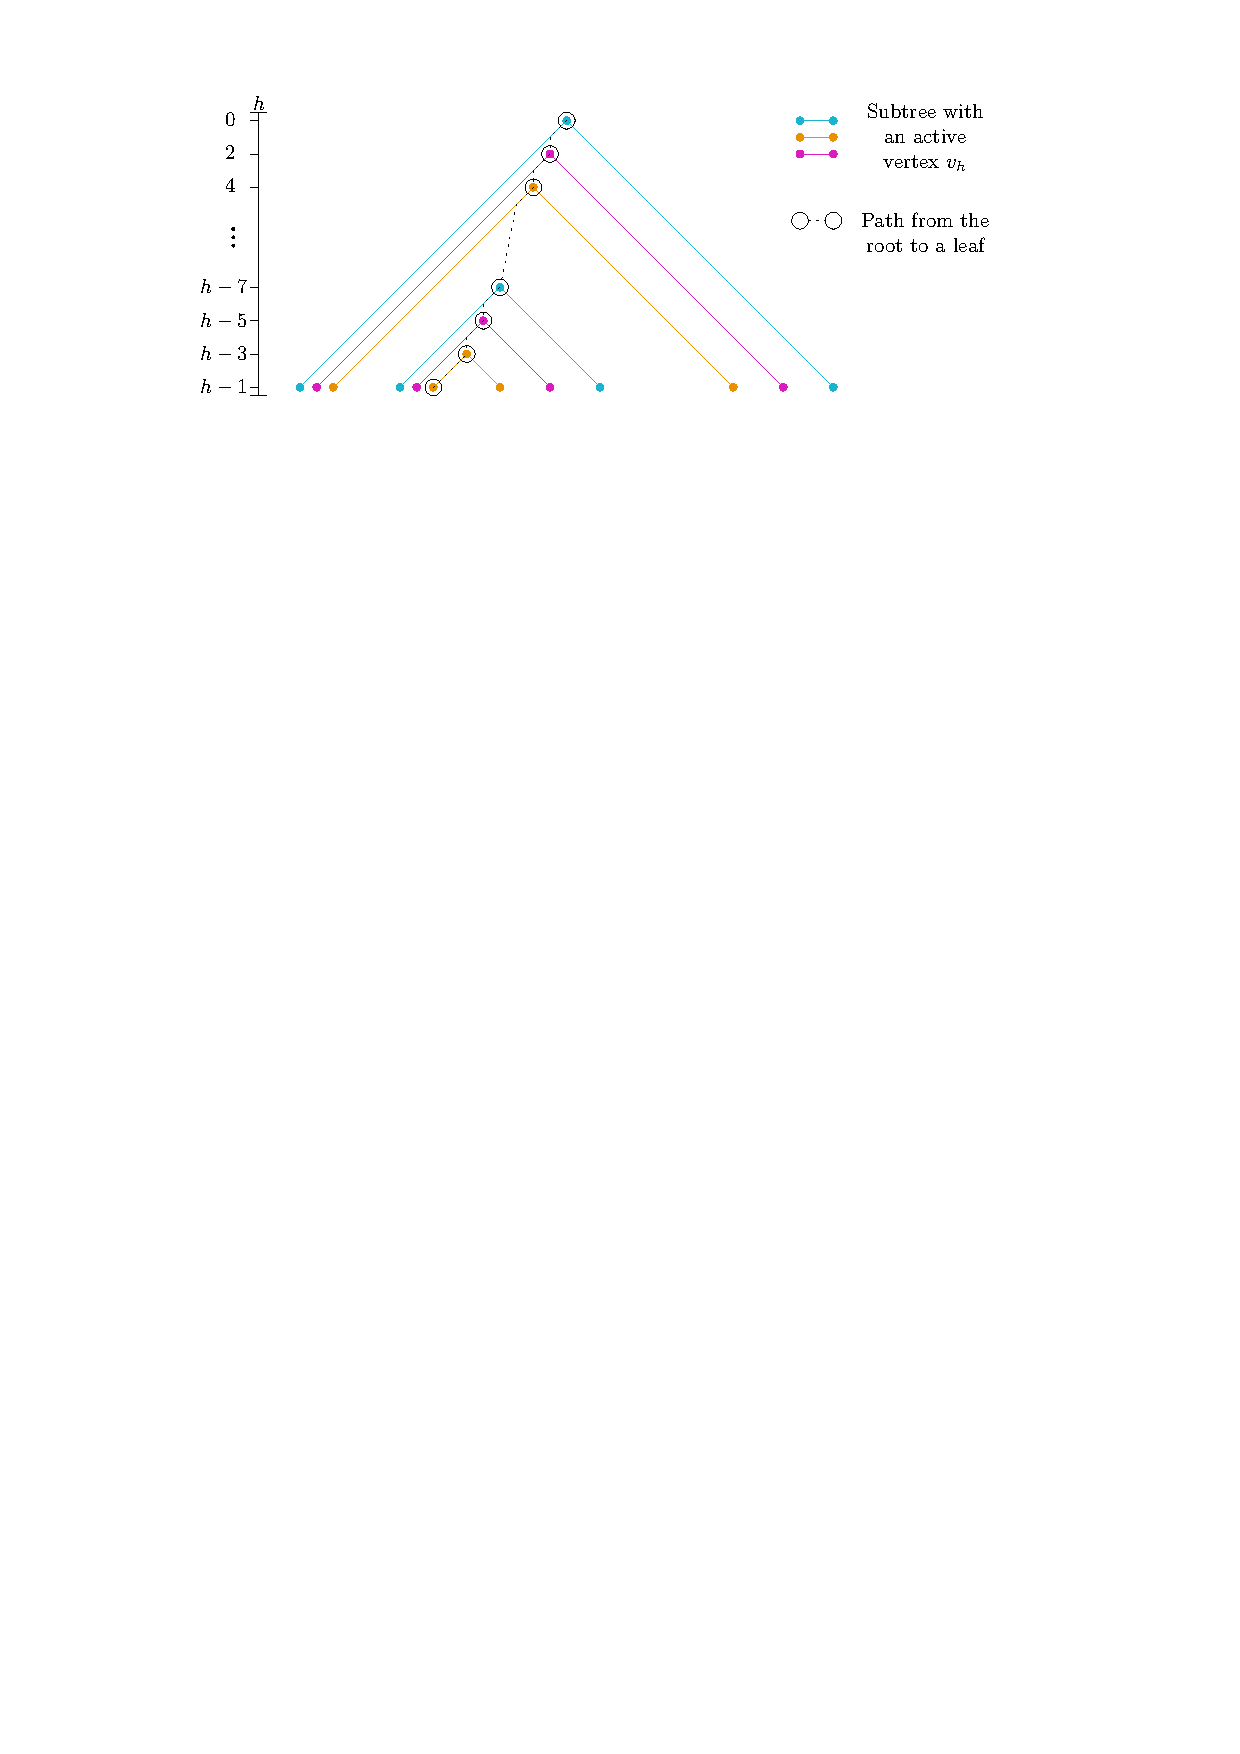
\includegraphics[page=1,width=0.9\linewidth]{graphics/active_vertices_log_n.pdf}
		\end{subfigure}
		\caption{A complete binary tree with up to $\mathcal{O}(\log n)$ active vertices for a DFS path}\label{im:active_vertices_log_n}
	\end{figure}

	Let $t'_r$ be the root and $t'_l$ a leaf of $T'$. Then, the path $p$ from $t'_r$ to $t'_l$ is unique. For every vertex $p_i$ of $p$, at most one vertex is set to being active during the DFS graph traversal, when starting at $t'_r$ up to $t'_l$. When $t'_l$ is explored, there are at most $\mathcal{O}(\log n')$ vertices still active. 
	The following holds for $p_i$ in $p$:
	\begin{itemize}
		\item If $p_i$ is a leaf and explored, then the induced new active vertex $v'_i\in V(G')$ is already finished since $|V(T'_{v'_i})| = 1$.
		\item If $p_i$ is not a leaf, then all the active vertices induced by exploring $p_{j}$ with $j>i$ are finished first when using DFS.
	\end{itemize}
	This means that up to $\mathcal{O}(\log n')$ vertices are active simultaneously when exploring $T'$.
\end{proof}

\begin{lemma}
	When prioritizing subtrees of minimal height while traversing any maximal outerplanar graph $G'$ with DFS, then there are up to $\mathcal{O}(\log^2 n')$ vertices active simultaneously.\label{l:maximal_outerplanar_log2_n_vercies_active}
\end{lemma}

\begin{proof}
	Let $G'$ be a maximal outerplanar graph with and $(T',W')$ be its tree decomposition. The height of $T'$ is bound by $\mathcal{O}(n')$. Since the degree of any vertex in $T'$ is at most 3, there are up to three binary trees connected to the root of $T'$. The minimal partitioning of the three binary subtrees $P_i = (\mathcal{T}_i,\mathcal{W}_i)$ of $T'$, $1\leq i \leq 3$, consist of binary tree partitions and $\mathcal{T}_i$ are binary trees.\\
	Consider a minimal partitioning $\mathcal{P}$ and a path $\tilde{t} = (t_1,...,t_k)$ starting at the root and ending at a leaf of $\mathcal{T}$. When subtrees of minimal heights are prioritized during every step of the DFS of $T$, then it holds that by the time the DFS reached a partition $t_j \in \tilde{t}$, then all the other partitions $t_i, i<j$ have been almost fully explored, leading to a constant amount of locally active vertices.\\
	In the case of $P$ being a complete binary tree, the priority of the subtree with the smallest height does not take any effect. Considering Lemma \ref{l:partition_binary_tree_lower_upper_bounds}, the largest upper bound for the height of $T$ lies in $\mathcal{O}(\log^2 n)$ when a minimal partitioning $P$ consists of $\sqrt{n'}$ partitions with $\sqrt{n'}$ vertices per partition bag and $\mathcal{T}$ being a complete binary tree. Analoguously to the proof of Lemma \ref{l:complete_maximal_outerplanar_log_n_active}, traversing a path from the root of $T$ to any leaf will set up to $\mathcal{O}(\log^2 n')$ vertices active.
\end{proof}

\subsection{Drawing Algorithm For Maximal Outerplanar Graphs With Two Bends}

Based on the fact that a layering induced by the drawing algorithm \ref{algo:complete_outerplanar_graph_dual} did improve the ratio for dense maximal outerplanar graphs, a new approach will create a box drawing with the layering property.\\
In order to draw a maximal outerplanar graph $G$, its tree decomposition will be transferred to an $SPQR$ tree.
\begin{lemma}
	A maximal SP-graph inherits a treewidth of 2.
\end{lemma}
\begin{proof}
	This follows by the recursive definition of maximal SP-graphs. The $K_3$ consists of three vertices and in its tree decomposition $(T,W)$, $T$ consists of one vertex, its bag of the three vertices defining the $K_3$. Adding a vertex $v$ adjacent to two already adjacent vertices $v_1,v_2$, a new vertex $t$ is added to $T$ with $\{v,v_1,v_2\}$ in its bag in $W$. Therefore, every bag contains exactly three vertices of $G$ and the treewidth of a maximal SP-graph values 2.
\end{proof}
\begin{lemma}
	There exists a function $f: (T,W) \to \mathcal{T}$ which derives an $SPQR$ tree out of a tree decomposition of a maximal SP-graph $G$ with the following properties:
	\begin{enumerate}
		\item There is no $R$ node in $\mathcal{T}$
		\item The skeleton of any serial node $S$ consists of exactly three vertices $s_1,s_2,s_3$
		\item The asymptotic height of $\mathcal{T}$ equals the asymptotic height of $T'$		
	\end{enumerate}\label{l:tree_decomp_to_SPQR}
\end{lemma}
\begin{proof}
	Let $G$ be an maximal SP-graph and $(T,W)$ its tree decomposition. Let $t_r$ be the root of $T$, representing a triangle of the vertices $v_1,v_2,v_3$. Its $SPQR$ tree $\mathcal{T}$ consists of three $Q$ vertices, one for every edge of the triangle, one $S$ node and one $P$ node. $\mathcal{T}$ is illustrated in the figure below:
	\begin{figure}[H]
		\begin{subfigure}{0.4\textwidth}
			\centering
			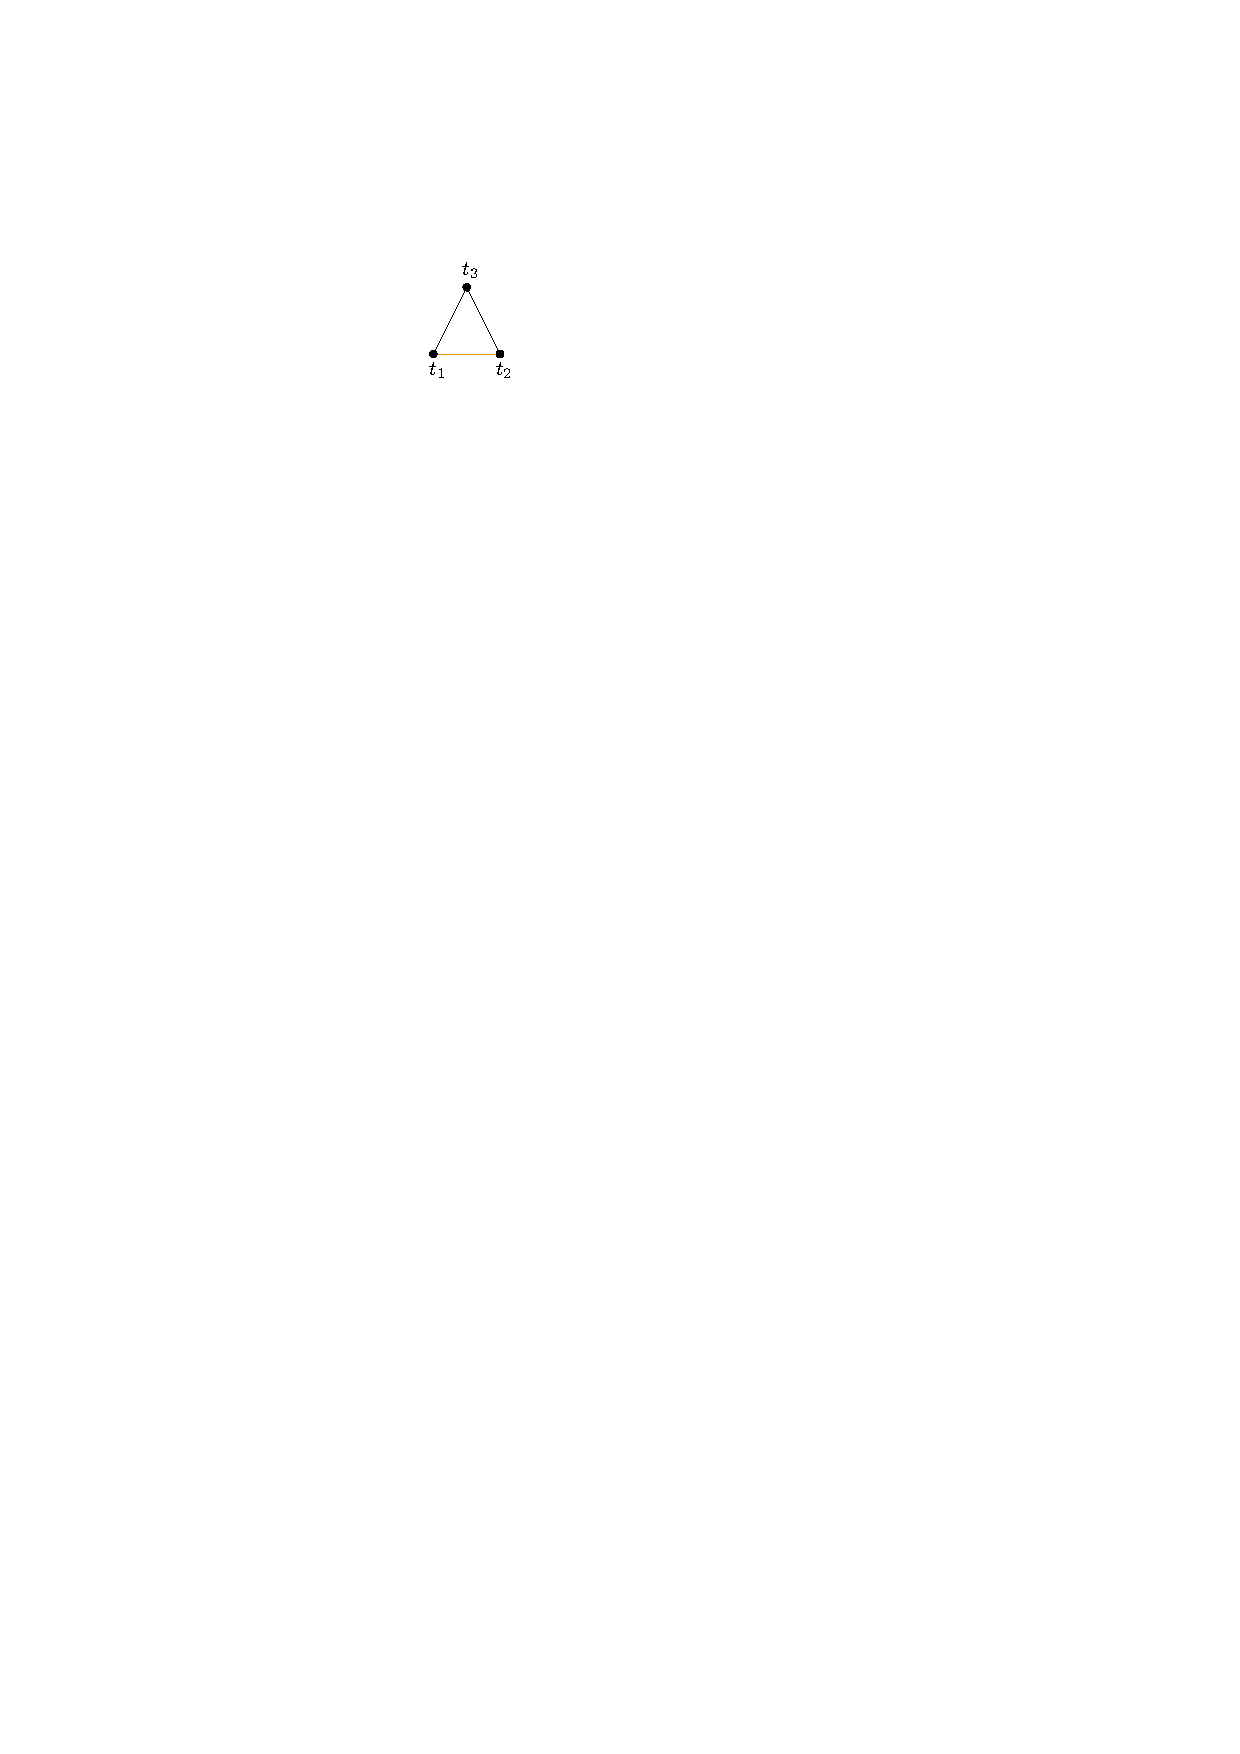
\includegraphics[page=1,width=0.7\linewidth]{graphics/SP_graphs_SPQR_inserting.pdf}
			\caption{A triangle}\label{im:SPQR_insert_a}
		\end{subfigure}
		\begin{subfigure}{0.4\textwidth}
			\centering
			\includegraphics[page=2,width=0.7\linewidth]{graphics/SP_graphs_SPQR_inserting.pdf}
			\caption{An $SPQR$ tree of \ref{im:SPQR_insert_a}}\label{im:SPQR_insert_b}
		\end{subfigure}
		\caption{A triangle illustrated in figure \ref{im:SPQR_insert_a} and its $SPQR$ tree in figure \ref{im:SPQR_insert_b}. The reference edge is marked in orange.}\label{im:SPQR_insert_1}
	\end{figure}
	When traversing $T$, every newly explored vertex of $T$ represents an addition of a new vertex of $G$ to $\mathcal{T}$. Let $v$ be the vertex of interest, adjacent to $v_1$ and $v_2$. $v_1$ and $v_2$ are already part of $\mathcal{T}$ and since the edge $(v_1,v_2)$ exists, there is a $Q$ node in $\mathcal{T}$ representing this edge. This $Q$ node is denoted as $Q(v_1,v_2)$. There are two cases to consider:
	\begin{description}
		\item[Case 1:] $Q(v_1,v_2)$ is adjacent to an $S$ node\\
		If $Q(v_1,v_2)$ is part of a serial composition in $\mathcal{T}$, adding $v$ will introduce a parallel composition around the split pair $(v_1,v_2)$ between $v$ and the residual graph $G\setminus\{v_1,v_2\}$. The following figure illustrates the insertion of $v$ into $\mathcal{T}$:
		\begin{figure}[H]
			\begin{subfigure}{\textwidth}
				\centering
				\includegraphics[page=3,width=\linewidth]{graphics/SP_graphs_SPQR_inserting.pdf}
			\end{subfigure}
			\caption{Insertion of a new vertex $v$ when $Q(v_1,v_2$ is not attached to a $P$ node)}\label{im:SPQR_insert_2}
		\end{figure}
		\item[Case 2:] $Q(v_1,v_2)$ is adjacent to $P(v_1,v_2)$\\
		Since there is already a parallel composition around the split pair $(v_1,v_2)$, inserting $v$ will be a serial composition as illustrated in the following figure:
		\begin{figure}[H]
			\begin{subfigure}{\textwidth}
				\centering
				\includegraphics[page=4,width=\linewidth]{graphics/SP_graphs_SPQR_inserting.pdf}
			\end{subfigure}
			\caption{Insertion of a new vertex $v$ when $Q(v_1,v_2$ is not attached to a $P$ node)}\label{im:SPQR_insert_2}
		\end{figure}
	\end{description}
	Since $G$ is a maximal SP-graph, there is not any $R$ node in $\mathcal{T}$ by definition. The second property holds as an invariant during the process of creating $\mathcal{T}$ since it is true for any triangle and any new vertex insertion. Every vertex of $T$ is substituted with a constant amount of vertices in $\mathcal{T}$, so the height of $\mathcal{T}$ equals the height of $T$ asympotically.\\
	So there exists a function $f$ which derives an $SPQR$ tree from a given tree decomposition with the stated properties.
\end{proof}
The drawing algorithm will transfer a tree decomposition $(T',W')$ of a maximal outerplanar graph $G'$ to an $SPQR$ tree $\mathcal{T}'$. Afterwards, the algorithm explores $\mathcal{T}'$ by DFS starting at the root node. This is achieved by a stack implementation in the pseudocode. For a vertex $t'\in V(\mathcal{T'})$, the child of $t'$ which roots the subtree of minimal height will always be prioritized during the DFS. This combined strategy of DFS and subtree priority will exclude unneccesarily inserted new layers in the resulting box drawing for $(T',W')$.\\
The following pseudocode creates a box drawing for a given $SPQR$ tree:\\
\begin{algorithm}[H]
	\caption{\texttt{DrawSPQR}$(\mathcal{T})$}\label{al:maximal_outerplanar_box_two_bends}
	\label{al:draw_SPQR}
	\KwIn{$SPQR$-tree $\mathcal{T}$ of a graph $G$}
	\KwOut{Box drawing $\mathcal{B}_G$}
	Stack \texttt{stack}\\
	\texttt{SPQRVerticesDone} $\gets \emptyset$\\
	$v \gets \mathcal{T}.\texttt{root}$
	% \tcc{$\mathcal{T}$ is rooted at a $Q$ node with vertices $q_1, q_2$}
	\texttt{stack.push}$(\mathcal{T}.\texttt{root})$\\
	\texttt{column} $\gets 0$\\
	$\delta \gets $ pairwise distance between layers\\
	\texttt{Lower Layer} $l_{low} \gets 0$\\
	\texttt{Upper Layer} $l_{up} \gets l_{low} + \delta$\\
	% \tcc{$l_{low}, l_{up}$ describe layers of interest for the remaining drawing}
	$B.\texttt{DrawBox}(q_1, l_{up}, \texttt{column})$\\
	$B.\texttt{DrawBox}(q_2, l_{low}, \texttt{column})$\\
	$\texttt{ActiveVertices} \gets \{q_1,q_2\}$\\
	\While{\texttt{VerticesDone} $\neq V(\mathcal{T})$}{
		$v\gets \texttt{stack.pop}$\\
		List \texttt{children} $\gets v\texttt{.children}$\\
		\texttt{children.SortByHeightOfSubtreesDescending}\\
		% \tcc{Every child of a vertex in $\mathcal{T}$ roots a subtree with its respective height}
		\While{\texttt{children} $\neq \emptyset$}{
			\texttt{stack.push(head(children))}
			\texttt{children.remove(head(children))}
		}
		\If(\tcp*{$Q$ node refers an edge $(q_1,q_2)$ of $G$}){$v$ is $Q$ node}{
			$B$\texttt{.DrawEdge}$((q_1,q_2),\texttt{column})$\\
			\If{$q_1$ finished}{
				\texttt{ActiveVertices.remove}$(q_1)$
			}
			\If{$q_2$ finished}{
				\texttt{ActiveVertices.remove}$(q_2)$
			}
			
		}
		\ElseIf{$v$ is $P$ node}{
			$\texttt{column} \gets \texttt{column}+1$\\
			\For{$v\in \texttt{ActiveVertices}$}{
				$B\texttt{.extendBox}(v)$
			}
			$l_{up} \gets layer(p_1)$\\
			$l_{low} \gets layer(p_2)$
		}
		\ElseIf(\tcp*{Serialization $S(s_1,s_2,s_3)$}){$v$ is $S$ node}{
			$\texttt{column} \gets \texttt{column}+1$\\
			\For{$v\in \texttt{ActiveVertices}$}{
				$B\texttt{.extendBox}(v)$
			}
			\If{$\nexists$ free layer between $layer(s_1)$ and $layer(s_3)$}{$l \gets B$\texttt.{addLayer}$(l_{up},l_{low})$}
			\Else{$l \gets $ free layer between $layer(s_1)$ and $layer(s_3)$}
			$B\texttt{.DrawBox}(s_2, l)$\\
			$\texttt{ActiveVertices.add}(s_2)$
		}
		\texttt{VerticesDone.add}$(v)$
	}
\end{algorithm}
The whole strategy is summed up in the following pseudocode:\\
\begin{algorithm}[H]
	\caption{\texttt{DrawMaximalOuterplanar}($G'$)}\label{al:maximal_outerplanar_two_bends}
	\KwIn{Maximal Outerplanar Graph $G'$}
	\KwOut{Polyline drawing $\Gamma_{G'}$ with two bends}
	$(T,W) \gets$ tree decomposition of $G'$ with lowest height\\
	$\mathcal{T'} \gets f(T',W')$\\
	$\delta \gets n$\\
	$\mathcal{B}_{G'} \gets \texttt{DrawSPQR}(\mathcal{T'})$\\
	$\Gamma_{G'} \gets \mathcal{B}_{G'}.\texttt{TransferToPolyline}$\\
	\Return $\Gamma_{G'}$
\end{algorithm}

\subsubsection{Analysis}

Algorithm \ref{al:maximal_outerplanar_two_bends} takes a maximal outerplanar graph $G'$ as input argument. Calculating the tree decomposition of $G'$ with lowest height runs in $\mathcal{O}(n)$ time since there are $\mathcal{O}(n)$ faces in $G'$. Transferring the tree decomposition to an $SPQR$ tree described by the function of Lemma \ref{l:tree_decomp_to_SPQR} takes $\mathcal{O}(|V(T')|) = \mathcal{O}(n)$ steps.\\
The drawing step described in Algorithm \ref{al:draw_SPQR} takes the $SPQR$ tree and creates a box drawing by iterating over its nodes. For the $SPQR$ tree $\mathcal{T}$, there are $\mathcal{O}(n)$ $P$, $S$ and $Q$ nodes, respectively. In case of a $Q$ node, drawing an edge takes constant time. In case of either a $P$ or a $S$ node, there are $\mathcal{O}(|\texttt{ActiveVertices}|)$ box extensions.\\
Transferring a box drawing to a polyline drawing includes the substitution of $\mathcal{O}(n)$ boxes with a grid point and $\mathcal{O}(n)$ edge reroutes over two bends per edge. The runtime therefore equals $\mathcal{O}(n\cdot |\texttt{ActiveVertices}|)$.

\begin{theorem}
	Let $G'$ be a complete maximal outerplanar graph. The drawing algorithm \ref{al:maximal_outerplanar_two_bends} produces a polyline drawing $\Gamma_{G'}$ on area $\mathcal{O}(n'^2 \log n')$ with two bends per edge and ratio $r \in \mathcal{O}(\log n')$, when the minimal distance between two layers is set to $n'$.\label{th:complete_maximal_outerplanar_ratio_logn}
\end{theorem}
\begin{proof}
	Consider the drawing algorithm \ref{al:maximal_outerplanar_box_two_bends}, producing a box drawing $\mathcal{B}_{G'}$. The algorithm first creates a tree decomposition of $G'$, $(T',W')$, and then uses DFS on $T'$ in its iteration to explore new active vertices which will be drawn in a potentially new layer. An active vertex $v$ blocks a layer of $\mathcal{B}_{G'}$ for further vertex insertions. When the DFS finished exploring the subtree $T'_{v}$ of $T'$, the layer of $v$ is availiable for new vertex insertions.\\
	Let $p$ be a path from the root of $T'$ to a leaf which creates the highest amount of layers. By Lemma \ref{l:complete_maximal_outerplanar_log_n_active}, there are up to $\mathcal{O}(\log n)$ vertices active during the DFS graph traversal of the tree decomposition of $G'$. Since $T'_{v}$ is a chain of vertices for any vertex $v\in V(G')$, there exists a subtree of $T'$ of asymptotically the same height as $T'_{v}$ which does not contain $v$ in its bags. After drawing $\mathcal{O}(\log n)$ vertices defined by $p$ on separate layers, the amount of layers created in $\mathcal{B}_{G'}$ suffice for the remaining drawing and is asympotitcally bound by $\mathcal{O}(\log n)$.\\
	The resulting box drawing therefore inherits $\mathcal{O}(\log n)$ layers with a pairwise distance of $n$. The height of the drawing is bound by $\mathcal{O}(n \log n)$. Since for every edge of $G'$ there exists a column in $\mathcal{B}_{G'}$, the width is bound by $O(n)$. The total area consumption therefore lies in $\mathcal{O}(n^2 \log n)$.\\
	When transferring the box drawing $\mathcal{B}_{G'}$ to a polyline drawing $\Gamma_{G'}$, every box $b_v$ is substituted with a grid point $v$ inside of $b_v$ and every edge incident to $b_v$ is rerouted by a bend point to the grid point for $v$. The polyline drawing produced by algorithm \ref{al:maximal_outerplanar_two_bends} inherits two bends per edge and has asymptotically the same area bound as the box drawing of algorithm \ref{al:maximal_outerplanar_box_two_bends}. The longest edge $l_{\max}$ spans the width and the height and its length is bound by $\mathcal{O}(n \log n) + \mathcal{O}(n) = \mathcal{O}(n \log n)$. The minimal Euclidian distance between to adjacent vertices values $n$ implied by the layering with its distance and the ratio therefore lies in $\mathcal{O}(\log n)$.
\end{proof}

\begin{theorem}
	Let $G'$ be a maximal outerplanar graph. The drawing algorithm \ref{al:maximal_outerplanar_two_bends} produces a polyline drawing $\Gamma_{G'}$ on area $\mathcal{O}(n'^2 \log^2 n')$ with two bends per edge and ratio $r \in \mathcal{O}(\log^2 n')$, when the minimal distance between two layers is set to $n'$.
\end{theorem}
\begin{proof}
	Considering Lemma \ref{l:maximal_outerplanar_log2_n_vercies_active}, up to $\mathcal{O}(\log^2 n')$ are active simultaneously when traversing the tree decomposition of $G'$ with DFS and prioritizing the subtrees of minimal height. Analouguously to the proof of Theorem \ref{th:complete_maximal_outerplanar_ratio_logn}, there are up to $\mathcal{O}(\log^2 n')$ layers inserted into the box drawing which will suffice for the whole drawing of $G'$. After transferring the box drawing to a polyline drawing, the resulting height lies in $\mathcal{O}(n\log^2 n)$. The width still lies in $\mathcal{O}(n)$. The ratio is therefore bound by $\mathcal{O}
	(\log^2 n')$. 
\end{proof}

\begin{theorem}
	There exists a class of maximal outerplanar graphs for which every graph admits a polyline drawing on $\mathcal{O}(n^2)$ area with a constant ratio.
\end{theorem}
\begin{proof}
	Let $G'$ be a maximal outerplanar graph with its partitioning $P = (\mathcal{P},\mathcal{W})$. Let $c$ be a constant so that for every partition $p_i \in \mathcal{P}$ it holds that $|w_i|\leq c, w_i \in \mathcal{W}$ and $\mathcal{P}$ be a chain of vertices of height $\mathcal{O}(n)$. Since the size of every partition is bound by $c$, the height of the regarding complete $k$-ary tree is bound by $\mathcal{O}(1)$.\\
	When $\mathcal{P}$ is a chain of vertices, the drawing algorithm \ref{al:maximal_outerplanar_two_bends} finishes a partition before proceeding to the next element of $\mathcal{P}$ due to the combined strategy of DFS and subtree priority. Since the amount of layers inserted into $\mathcal{B}_{G'}$ are determined by the amount of simultaneously active vertices, $\mathcal{B}$ inherits a constant amount of layers, resulting in a box drawing of $\mathcal{O}(n^2)$ area and a constant ratio.\\
\end{proof}

\subsubsection{Preserving Outerplanarity}

\begin{theorem}
	There exists an alternation of Algorithm \ref{al:draw_SPQR} that preserves the outerplanarity property of $\mathcal{G'}$ in a resulting box drawing $\mathcal{B}_{G'}$.
\end{theorem}
\begin{proof}
	Start at the root of $T'$, drawing a triangle on three layers. Without loss of generality, let $v_1$ be on the top layer, $v_2$ on the bottom layer and $v_3$ inbetween, placed left of the edge $(v_1,v_2)$.
	Since $G'$ is maximal outerplanar, by Lemma \ref{l:outerplanar_TD_properties} the three binary subtrees adjacent to the root of $T'$ address either $(v_1,v_2)$, $(v_1,v_3)$ or $(v_2,v_3)$. If a binary subtree refers to $(v_1,v_3)$, draw to the left inbetween the regarding layers. Analouguously for the binary tree referring to $(v_2,v_3)$. If a binary subtree refers the edge $(v_1,v_2)$, draw to the right. 
	
			\begin{figure}[H]
		\begin{subfigure}{\textwidth}
			\centering
			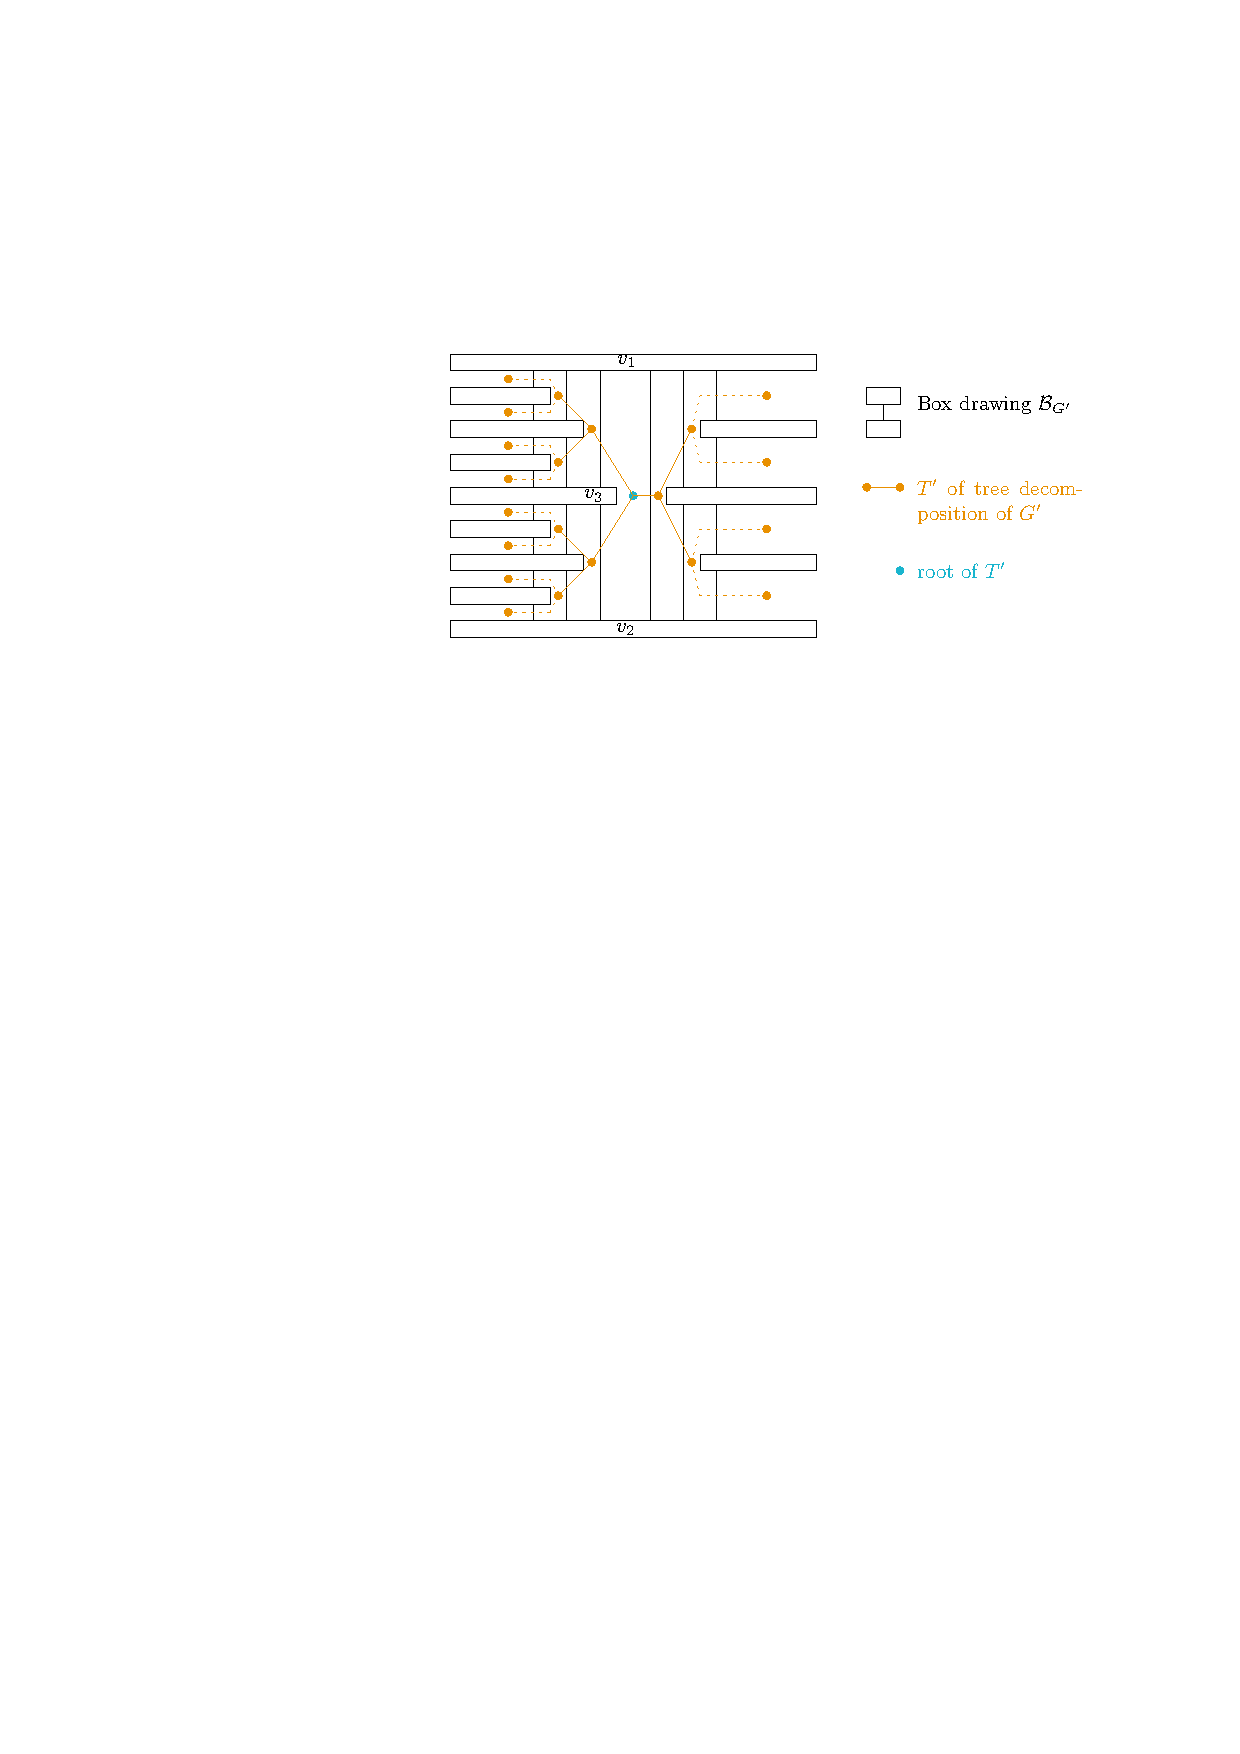
\includegraphics[page=1,width=\linewidth]{graphics/maximal_outerplanar_preserving_outerplanartiy_scheme.pdf}
		\end{subfigure}
		\caption{Scheme to draw a complete maximal outerplanar graph with preserving the outerplanarity property}\label{im:maximal_outerplanar_preserving_outerplanartiy_scheme}
	\end{figure}
	

	
	
	This way, every box lies on the outerface of $\mathcal{B}_{G'}$ and every vertex lies on the outerface in the resulting polyline drawing $\Gamma_{G'}$. The runtime, area consumption and ratio stay the same.
\end{proof}
\section{Series-Parallel Graphs}
% TODO What is this section about?

\section{Related Work}\label{section:related_work}
% TODO What is this section about?

\section{Future Work}\label{section:future_work}

\subsection*{Sharpness Of Ratio Upper Bound For Maximal SP Graphs}

As shown in section \ref{s:maximal_outerplanar}, the amount of simultaneously active vertices during a DFS graph traversal through a maximal outerplanar graphs tree decomposition lies in $\mathcal{O}(\log^2 n)$. One question is whether this upper bound is sharp. It might be possible to deduce the amount of active vertices of $G$ for a path from the root of the tree decomposition to any leaf. The consequence would be a significantally smaller area bound and ratio of any polyline drawing.

\subsection*{Polyline Drawing Implementation For Maximal SP Graphs}

An implementation of the drawing algorithm \ref{al:DrawMaximalSPGraph} would help evaluating the readability, aesthetics and the ratio of polyline drawings for large-scale maximal SP graphs. In order to implement the algorithm, it is necessary to guarantee consistent data structure representations regarding \emph{undirected graphs} and \emph{$SPQR$ trees} in a programming language of choice. Then, implementing the pseudocodes described in section \ref{s:maximal_outerplanar} and \ref{section:SP-graphs} would be straight-forward.

\subsection*{Drawing Approach For 3-trees}

Since in section \ref{section:related_work} it was illustrated that the layering approach based on a tree decomposition is not suitable for a ratio optimization for the class of 3-trees, a new approach for a polyline drawing algorithm is desirable.

\subsection*{General Drawing Algorithm For $k$-ary Trees}

The drawing algorithm \ref{al:complete_k-ary_tree} considers a $k$-ary tree to be complete in order to produce a straight-line drawing. While any $k$-ary tree admits a straight-line drawing with nearly-optimal ratio, the area consumption might behave exponentially if the $k$-ary tree is of height $\mathcal{O}(n)$. It would be desirable to construct a drawing algorithm for any input $k$-ary tree so that the area consumption of the resulting drawing stays reasonable and compact while not increasing the nearly-optimal ratio.
\section{Acknowledgements}
I would like to thank Prof. Michael Kaufmann and Henry Förster for instructing this final thesis. Further I appreciate helpful discussions with Dr. Michalis Bekos. I want to thank especially my parents for their patience and encouragement despite hardest family issues. A special thanks goes to Thomas Stüber, who made me appreciate the theoretical field of computer science.
%\begin{thebibliography}{9}
	\bibitem{SMOG}
	Smooth Orthogonal Layouts,
	\textit{Journal of Graph Algorithms and Application vol. 17, p.~575-595}\\
	Bekos, Kaufmann, Kobourov, Symvonis,
	2013.
	\bibitem{SMOcti_rel}
	On Smooth Orthogonal and Octilinear Drawings:
	\textit{Relation, Complexity and Kandinsky Drawings}\\
	Bekos, Förster, Kaufmann,
	submitted September 2017.
	\bibitem{SMOcti}
	On Smooth Orthogonal and Octilinear Drawings, \textit{Preprint Edition}\\
	Bekos, Förster, Kaufmann.
	\bibitem{Ortho}
	Planar Orthogonal and Polyline Drawing Algorithms,
	\textit{Handbook of Graph Drawing and Visualization,, page 223-245},
	Duncan, Goodrich,
	2013.
	\bibitem{slideplayer}
	Constraints In Orthogonal Graph Drawing, Stroh, Retrieved from \url{http://slideplayer.org/slide/660000/}, March 2018.
	\bibitem{podevsaef}
	The Effect Of Almost-Empty Faces On Planar Kandinsky Drawings, Bekos, Kaufmann, Krug, Siebenhaller\\
	online June 2015.
\end{thebibliography}
\printbibliography
\end{document}